\documentclass[11pt, a4paper, oneside]{book}

\usepackage{fancyhdr}
\pagestyle{fancy}
\fancyhf{}

\usepackage[english]{babel}
\usepackage{graphicx}
\usepackage[colorlinks,hyperindex,plainpages=false,breaklinks]{hyperref}
\usepackage{amssymb}
\usepackage{wasysym} 
\usepackage{wrapfig}
\usepackage{enumerate}
\usepackage{placeins} % Necessary for \FloatBarrier
\usepackage{subfig}   % Necessary for subfloat (images next to each other)
\usepackage{color}
\usepackage[usenames,dvipsnames,svgnames]{xcolor}
\usepackage{listings}

\definecolor{codelightgray}{rgb}{0.87,0.87,0.87}

\hypersetup{colorlinks=true,% 
	linkcolor=black,%
	citecolor=red,%
	filecolor=blue,% 
	menucolor=black,% 
	pagecolor=black,%
	urlcolor=black
}

\lstset{language=,
    keywordstyle=\color{blue},
    basicstyle=\scriptsize\ttfamily,
    showstringspaces=false,
    backgroundcolor=\color{codelightgray},
    morekeywords={SELECT,FROM,WHERE,AND,OR,EClass}
}

% TOC depth
\setcounter{tocdepth}{1}

\setlength{\parindent}{0pt} 
\setlength{\parskip}{0.3cm}

% Remove section numbers 0.1, 0.2 ..
\renewcommand{\thesection}{\arabic{section}} 

\graphicspath{%
{../../06_miscellaneous/commonFiles/}% Title image and memBox illustration
{../1_gettingStarted/}{../1_gettingStarted/visImportImages/}{../1_gettingStarted/texImportImages/}%
{../2_schema/}{../2_schema/visSImages/}{../2_schema/texSImages/}%
{../3_rules/}{../3_rules/visRImages/}{../3_rules/texRImages/}%
{../4_inAction/aImages/}%
{../5_integrator/}%
{../6_extendingTransformation/splashImages/}{../6_extendingTransformation/visProtoImages/}{../6_extendingTransformation/texProtoImages/}%
{../7_sychronization/}%
}

% --- HEADER FUNCTIONS % --------------------------------------------------------------------------------------------------------------------------------------
% Default plain header; turn off all lines and colors; turn on page numbers for all
\newcommand{\noHeader}{
	\fancyfoot{}
 	\fancyhead[R]{\thepage}
	\fancyhead[L]{}
	\renewcommand{\headrulewidth}{0pt}
}

% Common instruction Header; Black
\newcommand{\genHeader}{
	\fancyfoot{}
	\fancyhead[L]{}
	\renewcommand{\headrulewidth}{1.5pt}
 	\renewcommand{\headrule}{\hbox to\headwidth{%
  		\color{Black}\leaders\hrule height \headrulewidth\hfill}}
}

% Visual instructions; Red header
\newcommand{\visHeader}{
	\fancyfoot{}
	\fancyhead[L]{\color{RedOrange}\tiny \bf VISUAL}
	\renewcommand{\headrulewidth}{1.5pt}
	\renewcommand{\headrule}{\hbox to\headwidth{%
  		\color{RedOrange}\leaders\hrule height \headrulewidth\hfill}}
}

% Text instructions; Blue header
\newcommand{\texHeader}{
	\fancyfoot{}
	\fancyhead[L]{\color{CornflowerBlue}\tiny \bf TEXTUAL}
	\renewcommand{\headrulewidth}{1.5pt}
	\renewcommand{\headrule}{\hbox to\headwidth{%
  		\color{CornflowerBlue}\leaders\hrule height \headrulewidth\hfill}}
}
% -------------------------------------------------------------------------------------------------------------------------------------------------------------

\newcommand{\requiredTime}[1]{ {\scriptsize \texttt{Approximate time to complete: #1} } }

% Jump links 
\newcommand{\jumpSingle}[1]{
\fancyfoot[OR]{$\triangleright$ \hyperlink{#1}{\texttt{Next}}}
}

\newcommand{\jumpDual}[2]{
\fancyfoot[RO]{ $\triangleright$ \hyperlink{#1}{\texttt{Next [visual]\hspace{0.2cm}}}%
 \\ $\triangleright$ \hyperlink{#2}{\texttt{Next [textual]}}}
}

% These words should appear in the glossary
\newcommand{\define}[1]{ \marginpar{\small\emph{#1}} }

% Text syntax/command format
\newcommand{\syntax}[1]{ \begin{quote} \small \texttt{#1} \end{quote}}	

% Quick author note; remove from final
\newcommand{\update}{{\bf update }}

% TODO: update description download link
\newcommand{\dlPartZero}{\url{www.emoflon.org}}

% TODO:  Update version number (Title Page Information)--------------------------------------------------------------------------------------------------------
\def\partTitle{Part IV: Triple Graph Grammars}
\def\versionNumber{0.1}
\title{
\flushright
{\LARGE\bfseries An Introduction to Metamodelling\\
and Graph Transformations}
\noindent\rule[-1ex]{\textwidth}{5pt}\\[2.5ex]
\hfill\emph{\LARGE\bfseries with eMoflon}
\flushleft
{\small Version 2.1}
\flushright

\includegraphics[width=0.85\textwidth]{pics/eMoflon3} 
}

\date{}  
\author{} 

\begin{document}

\frontmatter 
\noHeader

% Title Page without following blank page
{\let\newpage\relax\maketitle}

% Copyright notice
\begin{small} 
Copyright \copyright~2011--\the\year{} Real-Time Systems Lab, TU Darmstadt.
Anthony Anjorin, Erika Burdon, Frederik Deckwerth, Roland Kluge, Marius Lauder,
Erhan Leblebici, Daniel T\"ogel, David Marx, Lars Patzina, Sven Patzina, Alexander Schleich, Sascha Edwin Zander, Jerome Reinl\"ander, Martin Wieber, and contributors.
All rights reserved.

This document is free; you can redistribute it and/or modify it under the terms of the GNU Free Documentation License as published by the Free Software Foundation; either version 1.3 of the License, or (at your option) any later version.
Please visit \href{http://www.gnu.org/copyleft/fdl.html}{http://www.gnu.org/copyleft/fdl.html} to find the full text of the license.
 
% TODO Remove this?? It can be found easily online .. (we can even offer it on
% the download page) For your convenience, this document includes a copy of the \emph{GNU General Public License} starting from page~\pageref{chap:gpl}.
  
For further information contact us at \eMoflonContact.
  
\vskip3cm
\textit{The eMoflon team}\\
Darmstadt, Germany (\monthword{\month} \the\year)
\end{small}
\let\cleardoublepage\clearpage

% TOC
\tableofcontents

% Store page counter
\newcounter{romanpages}
\setcounter{romanpages}{\value{page}}

\mainmatter

% Main content for this Part 
\vspace*{2cm}

{\bf \huge Part IV:}
\vspace{1cm}

{\bf \Huge Learning Box to Dictionary \\ \emph{and} back again with TGGs }
\vspace{1cm}

\genHeader
\label{chap:Learning-Box-to-Dictionary-and-Back-Again}

If you're just joining us in this part and are only interested in bidirectional model transformations with \emph{Triple Graph Grammars} then welcome! 
In fact to keep things simple, we shall assume for the tool-related parts of the handbook that you're starting (over) with a clean slate. 

To briefly review what we have done so far in the previous parts of this handbook: we have developed Leitner's learning box by specifying its \emph{abstract syntax} and \emph{static semantics} as a
\emph{metamodel}, and finally implementing its \emph{dynamic semantics} via Story Driven Modeling (programmed graph transformations). If the previous sentence
could just as well have been in Chinese\footnote{Replace with Greek if you are chinese.  If you are chinese but speak fluent Greek, then we give up. You get the
point anyway, right?} for you, then consider work through Parts I---III.
If you're only in interested in TGGs, however, and you have the appropriate background (or don't care) then that's also fine.

Even though SDMs are crazily cool (don't you forget that!), it is deeply unsatisfactory implementing an inherently \emph{bidirectional} transformation as two unidirectional transformations. 
If you critically consider the straighforward solution of specifying forward and backward transformations as separate SDMs, you should be able to realise at least the following problems:

\vspace{-0.5cm}

\begin{description}
\item[Productivity:] We have to implement two transformations that are really quite similar, \emph{separately}. This simply doesn't feel productive.
Wouldn't it be nice to implement one direction such as the forward transformation, then get the backward transformation for free? How about deriving
forward \emph{and} backward transformations from a common joint specification?

\item[Maintainability:] Another maybe even more important point is that two separate transformations often become a pain to maintain and keep
\emph{consistent}. If the forward transformation is ever adjusted to produce a different target structure, the backward transformation must be updated
appropriately to accommodate the change, and vice-versa.  Again, it would be great if the language offered some support.

\item[Traceability:] Finally, one often needs to identify the reason why a certain object has been created during a transformation process. This increases the
trust in the specified transformation and is essential for working with systems that may actually do some harm (i.e., automotive or medical systems). With two
separate transformations, \emph{traceability} has to be supported manually (and that seriously sucks)! 

\item[Incrementality and other cool stuff:] Traceability links can also be used to propagate changes made to an existing pair of models \emph{incrementally}, i.e., without recreating the models from scratch. 
This is not only more efficient in most cases (small change and humongous models), but is also sometimes necessary to avoid losing information in one model that simply cannot be recreated with the other model.
Finally, having a declarative (meaning here direction-agnostic, i.e., neither forward nor backward) specification makes it easier to derive all kind of different transformations including a model generator (we'll actually get to use this later).
\end{description}

Our goal in this part is, therefore, to investigate how Triple Graph Grammars (TGGs), a cool \emph{bidirectional} transformation language, can be used to address these problems. 
To continue with our running example, we shall transform \texttt{Leit\-ners\-Learn\-ing\-Box}, a partitioned container populated with unsorted cards that are moved through the box as they are memorized,\footnote{For a detailed review on Leitner's Learning Box, see Part II, Section 1} into a \texttt{Dictionary}, a single flat container able to hold an unlimited number of entries classified by difficulty (\Cref{fig:transformIdea}).

\begin{figure}[htbp]
\begin{center}
  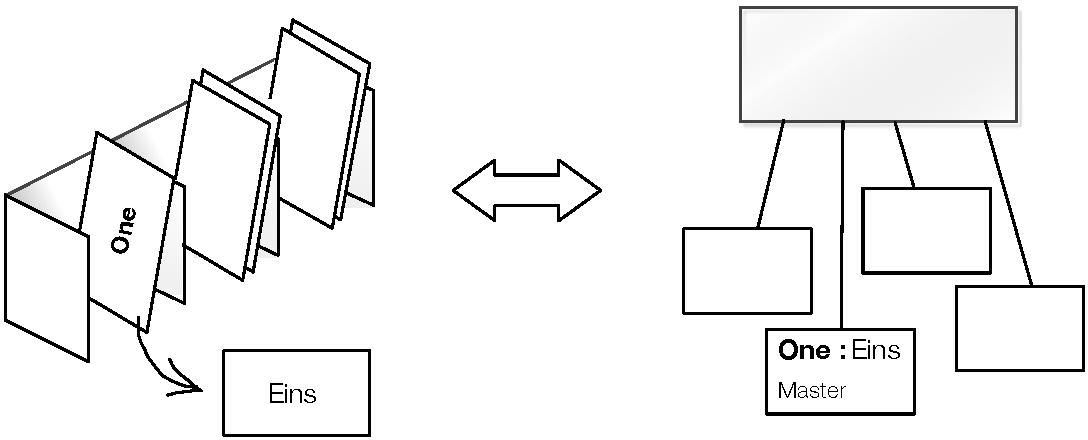
\includegraphics[width=\textwidth]{TGGTransformationExample.pdf}
  \caption{Transforming Leitner's learning box into a dictionary}
  \label{fig:transformIdea}
\end{center}
\end{figure}

To briefly explain, each card in the box has a keyword on one side (called \emph{face}) that a user can see, paired with a definition hidden on the opposite side (called \emph{back}). 
We will combine each of these to create the keyword and content of a single dictionary entry, perhaps assigning a difficulty level based on the card's current position in the box. 
We also want to be able to transform in the opposite direction, transforming each dictionary entry into a card by splitting up the contents, and inserting the new element into a specific partition in the box. 
After a short introduction to TGGs and setting up your workspace correctly, we shall see how to develop
your first bidirectional transformation!


%%% Local Variables: 
%%% mode: latex
%%% TeX-master: "TGG_mainFile"
%%% End: 


\section{Triple Graph Grammars in a nutshell}
\label{sec:nutshell}
\genHeader

Triple graph grammars~\cite{tgg:schuerr_94,sk2008,Klar2010} are a declarative, rule-based technique of specifying the simultaneous evolution of three connected
graphs. Basically, a TGG is just a bunch of rules. Each rule is quite similar to a \emph{story pattern} and describes how a graph structure is to be built-up
via a precondition (LHS) and postcondition (RHS). The key difference is that a TGG rule describes how a \emph{graph triple}\define{Graph Triples} evolves, where
triples consist of a source, correspondence, and target component. This means that executing a sequence of TGG rules will result in source and target graphs
connected via nodes in a third (common) correspondence graph.

\vspace{0.25cm}

Please note that the names ``source'' and ``target'' are arbitrarily chosen and do not imply a certain transformation direction. Naming the graphs ``left'' and
``right'', or ``foo'' and ``bar'' would also be fine. The important thing to remember is that TGGs are \emph{symmetric} in nature.

\vspace{0.25cm}

So far, so good! Except you may be now be asking yourself the following question: ``What on earth does all this have to do with bidirectional model
transformation?'' There are two main ideas behind understanding TGGs:

\begin{description}

\item[(1) A TGG defines a consistency relation:]% 
Given a TGG (a set of rul\-es), you can inspect a source graph $S$ and a target graph $T$, and say if they are \emph{consistent} with respect to the TGG. How?
Simply check if a triple ($S\leftarrow C\rightarrow T$) can be created using the rules of the TGG!

\vspace{0.25cm}

If such a triple can be created, then the graphs are consistent, denoted by: $S \Leftrightarrow_{TGG} T$. This consistency relation can be used to check if a
given bidirectional transformation (i.e., a unidirectional forward ($f$) and backward ($b$) transformation) is correct. In summary, \emph{A TGG can be viewed as
a specification of how the transformations \emph{should} behave ($S \Leftrightarrow_{TGG} f(S)$ and $b(T) \Leftrightarrow_{TGG} T$)}.
	
\item[(2) The consistency relation can be operationalized:]% 
This is the surprising (and extremely cool) part of TGGs -- forward \emph{and} backward rules (i.e., $S$ or $T$) can be derived automatically from every TGG
rule~\cite{Giese2010,Hermann2011a}! 

\vspace{0.25cm}

In other words, the description of the simultaneous evolution of the source, correspondence, and target graphs is \emph{sufficient} to derive a forward and
a backward transformation. As these derived rules explicitly state step-by-step how to perform forward and backward transformations, they are called
\emph{operational} rules as opposed to the original TGG \emph{declarative} rules specified by the user. This derivation process is therefore also referred to
as the\define{Operationalization}\emph{operationalization} of a TGG.
	
\end{description}

Before getting our hands dirty with a concrete example, here are a few extra points for the interested reader:  

\begin{itemize}

\item Many more operational rules can be automatically derived from the $S \Leftrightarrow_{TGG} T$ consistency relation including inverse rules to \emph{undo}
a step in a forward/backward transformation~\cite{LAVS_ICGT_2012},\footnote{Note that the TGGs are symmetric and forward/backward can be interchanged freely.
As it is cumbersome to always write forward/backward, we shall now simply say forward.} and rules that check the consistency of an existing graph triple.

\item You might be wondering why we need the correspondence graph. The first reason is that the correspondence graph can be viewed as a set of explicit
traceability links, which are nice to have in any transformation. With these you can, e.g., immediately see which elements are related after a forward
transformation. There's no guessing, no heuristics, and no interpretation or ambiguity.

\vspace{0.25cm}

The second reason is more subtle, and difficult to explain without a concrete TGG, but we'll do our best and come back to this at the end. The
key idea is that the forward transformation is very often actually \emph{not} injective and cannot be inverted! A function
can only be inverted if it is \emph{bijective}, meaning it is both \emph{injective} and \emph{surjective}. So how can we derive the backward
transformation?

\vspace{0.25cm}

eMoflon sort of ``cheats'' when executing the forward transformation and, if a choice had to be made, remembers what target element was chosen. In this way,
eMoflon \emph{bidirectionalize}s the transformation on-the-fly with correspondence links in the correspondence graph. The best part is that if the
correspondence graph is somehow lost, there's no reason to worry because the \emph{same} TGG specification that was used to derive your forward transformation
can also be used to reconstruct a possible correspondence model between two existing source and target models.\footnote{We refer to this type of operational
rule as \emph{link creation}}

\end{itemize}
This was a lot of information to absorb all at once, so it may make sense to re-read this section after working through the example. In any case, enough theory!
Grab your computer (if you're not hugging it already) and get ready to churn out some TGGs!


% Setting up (or starting fresh)
\newpage
\section{Setting up your workspace}
\genHeader

Before you're able start any TGG transformation, you need to have two metamodels -- a source and target -- already prepared. Our source will be Leitner's
Learning Box, a partitioned container populated with cards. Each card has a keyword on its back, and a definition on its face. It is specified in
\texttt{LearningBoxLanguage}, fully built and completed in Parts II and II. Conversely, our target metamodel will be a Dictionary, a single container object
able to hold an unlimited number of entries. The goal is to have one dictionary per topic, where each entry would have a main keyword, and some relevant content. 

So how do we hope to transform a learning box into a dictionary, and vice versa? The first goal, from \texttt{BoxToDictionary}, is to combine each side of the
card as a single entry's content, then insert it anywhere into a dictionary. In the other direction, we want to be able to sort a series of entires based on
their difficulty level, in addition to splitting up their content into a useful keyword or question, and answer.

If you've just joined us in the handbook, complete Section~\ref{sec:loadSourceMeta} to load the preprepared \texttt{LeitnersLearningBox} metamodel into your
workspace. If your source metamodel is ready to go, skip ahead to  either \texttt{\hyperlink{sec:multiEAP}{Section 2.2 (Visual)}}
or~\texttt{\hyperlink{sec:multiMOSL}{Section 2.3 (Textual)}} to import \texttt{DictionaryLanguage} into your workspace. Please note that these instructions for
properly importing the metamodel into the same project are crucial as both metamodels must be in the same project in order to properly specify an integration
with TGGs.

\subsection{Starting Fresh}
\label{sec:loadSourceMeta}
\begin{itemize}

\item[$\blacktriangleright$] To get started, press the \texttt{new} button on the toolbar and navigate to ``Examples/eMoflon Handbook Examples/''
(Fig.~\ref{fig:downPartIV}).  We have created two `cheat' packages based on eMolfon's specification types --  pick the one you would prefer to use.\footnote{For
a brief discussion on the differences between the two, refer to Part I, Section I} They both contain the finished metamodel, complete with all objects,
references, and implemented SDMs as completed in the previous parts.

\item[$\blacktriangleright$] After loading, if your package explorer does not look similar to ours in Fig.~\ref{fig:workingSets} with at least two distinct
nodes, select the small, downward facing arrow in the corner of the module window. Choose ``Working Sets/Top Level Elements.'' We use these to structure the
workspace in Eclipse.

\end{itemize}

At this point we recommend reading the introduction to Part II for an overview of \texttt{LeitnersLearningBox}, it's purpose and goals, and how \texttt{card}s
are moved between each \texttt{partition}. Hopefully background will help you better understand the steps in \emph{this} part, as we're continuing to build on
that idea. 

\begin{figure}[htbp]
\begin{center}
  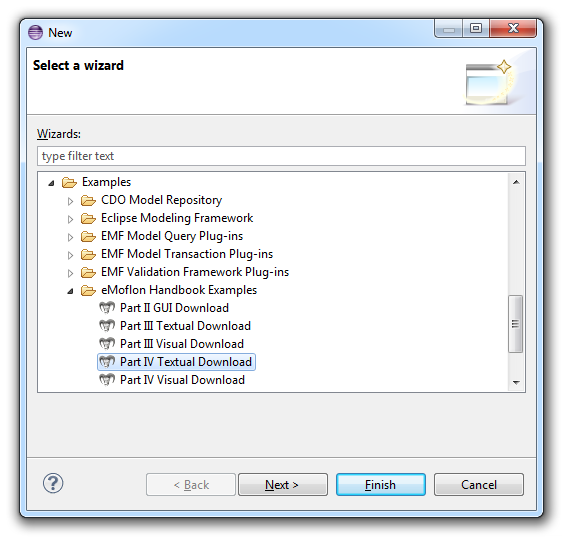
\includegraphics[width=0.8\textwidth]{eclipse_downloadWizardPartIV}
  \caption{Download a file set to get started}
  \label{fig:downPartIV}
\end{center}
\end{figure}

\vspace{0.5cm}

% Forced placement so it would co-operate
\begin{figure}[h!]
	\centering
  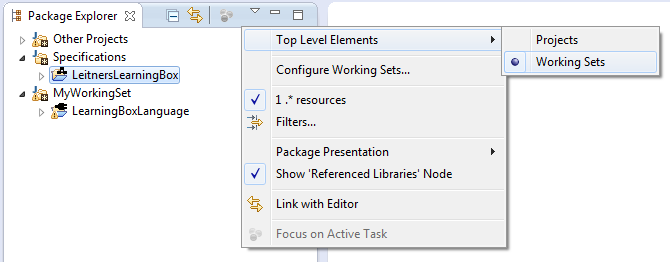
\includegraphics[width=0.9\textwidth]{eclipse_workingSets}
	\caption{Setting your Package Explorer}
	\label{fig:workingSets}
\end{figure}

\jumpDual{sec:multiEAP}{sec:multiMOSL}

% Instructions for loading target model
\newpage
\hypertarget{multiEAP}{}
\subsection{Importing and working with multiple EAPs}
\visHeader

Please note that the following instructions on how to properly export and import Enterprise Architect (EA) files are \emph{not} an eMoflon-exclusive feature.
We have included them here as part of our handbook as getting this right is crucial for working with eMoflon, especially when working with TGGs. The main
problem is that, as far as we know, EA does not (yet) support referencing model elements in one EAP from another, completely different EAP. This means that all
required metamodels have to first be merged in the same EAP before such references can be specified (as required for TGGs).

\begin{itemize}

\item[$\blacktriangleright$] Press the \texttt{new} button in the Eclipse toolbar and navigate to ``Examples/eMoflon Handbook Examples/''
(Fig.~\ref{eclipse:dictionaryDownloadWizard}). Find and select \texttt{Part IV Visual Dictionary Language} to copy a new \texttt{Dict\-ion\-ary\-Lang\-uage}
metamodel project into your workspace.

\vspace{0.5cm}

% Image stored in ../1_gettingStarted/textImportImages/  (repeated image)
\begin{figure}[htbp]
\begin{center}
  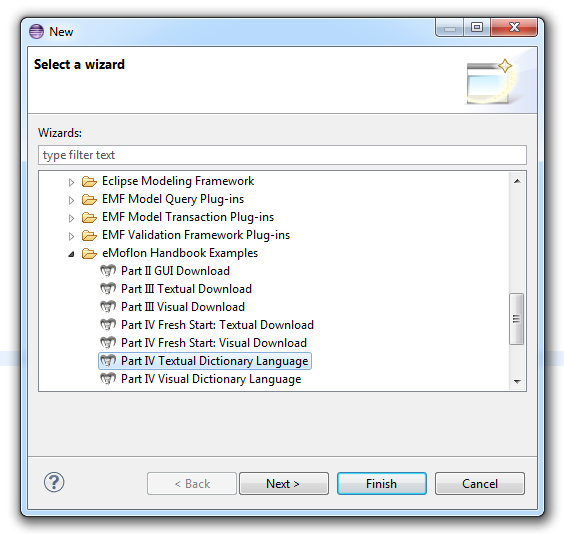
\includegraphics[width=0.8\textwidth]{eclipse_part4DictionaryLanguageDownload}
  \caption{Get the visual \texttt{DictionaryLanguage} metamodel}
  \label{eclipse:dictionaryDownloadWizard}
\end{center}
\end{figure}

\item[$\blacktriangleright$] If successful, your workspace should resemble Fig.~\ref{eclipse:loadedDictionaryEAP}. Double-click
\texttt{Dictionary.eap} to open it in EA.

\newpage

\begin{figure}[htbp]
\begin{center}
  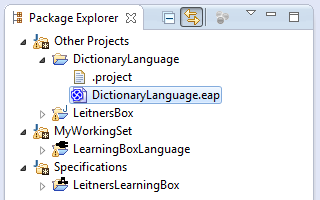
\includegraphics[width=0.5\textwidth]{eclipse_loadedDictionaryEAP}
  \caption{\texttt{Dictionary} metamodel successfully copied into the workspace}
  \label{eclipse:loadedDictionaryEAP}
\end{center}
\end{figure}

\item[$\blacktriangleright$] The file's project browser should resemble Fig.~\ref{ea:dictionaryLangStart}. Feel free to inspect the main
\texttt{DictionaryLanguage} diagram until you're familiar with the metamodel. Our work will be focused on the \texttt{Dictionary} and \texttt{Entry} classes.
You'll be able to see that dictionaries can be assigned unique \texttt{EString title}s, and each entry will have some sort of \texttt{content} matched with one
of three difficulty \texttt{level}s.

\vspace{0.5cm}

\begin{figure}[htbp]
\begin{center}
  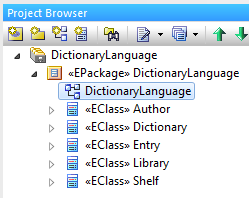
\includegraphics[width=0.4\textwidth]{ea_dictLangProBrowser}
  \caption{The \texttt{DictionaryLanguage} metamodel structure}
  \label{ea:dictionaryLangStart}
\end{center}
\end{figure}

\item[$\blacktriangleright$] It should be said that while you are able to simply copy and paste packages between multiple EAPs (i.e., copy
\texttt{<<E\-Pack\-age>>Dict\-ion\-ary\-Lang\-uage} into the \texttt{MyWorkingSet} root note of your source metamodel), if any of the copied packages have
dependencies on other packages, it cannot be done so easily. All links would be destroyed! 

\clearpage

\item[$\blacktriangleright$] Therefore, to properly migrate the \texttt{DictionaryLanguage} package, right-click on the EPackage root, navigate to
``Import/Export" and select \texttt{Export Model to XMI\ldots} (Fig.~\ref{ea:contextExport}). Alternatively, you can select the root in the project browser and
press \texttt{Ctrl + Alt + E}.

\vspace{0.5cm}

\begin{figure}[htbp]
\begin{center}
  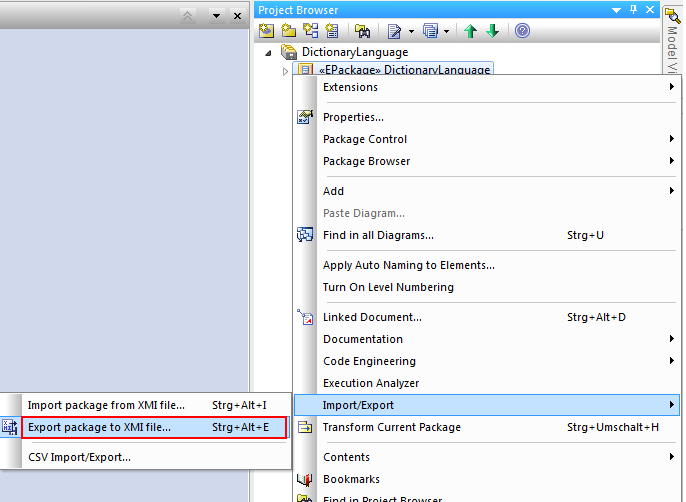
\includegraphics[width=\textwidth]{ea_contextExport}
  \caption{Starting the export process in EA}
  \label{ea:contextExport}
\end{center}
\end{figure}

\item[$\blacktriangleright$] Switch the export type to \texttt{XMI 2.1} in the dialogue and save the file somewhere easily accessible. Press export, and close
the window once the small green bar appears (Fig.~\ref{ea:export}).

\begin{figure}[htbp]
\begin{center}
  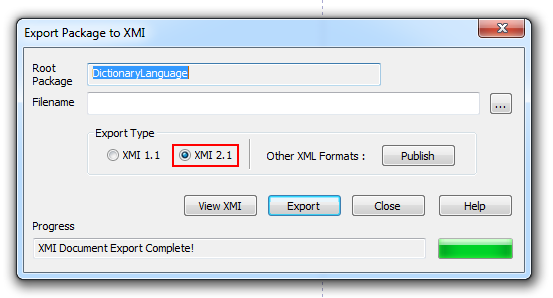
\includegraphics[width=0.9\textwidth]{ea_dialogueExport}
  \caption{Exporting the metamodel to a file}
  \label{ea:export}
\end{center}
\end{figure}

\item[$\blacktriangleright$] Go back to Eclipse and open \texttt{LeitnersLearningBox.eap}. Right-click on \texttt{MyWorkingSet} and navigate to ``Import
Model from XMI\ldots''

\item[$\blacktriangleright$] Find the \texttt{.xmi} file you just saved and press \texttt{import}. Press \texttt{OK} in the confirmation dialogue; Your project
browser should now resemble Fig.~\ref{ea:importProBrowser}, with both metamodels in the same working set, in the same EAP.

\begin{figure}[htbp]
\begin{center}
  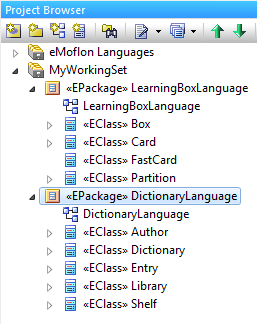
\includegraphics[width=0.5\textwidth]{ea_loadedDictionaryMetamodel}
  \caption{The TGG metamodels successfully included in one EAP}
  \label{ea:importProBrowser}
\end{center}
\end{figure}

\clearpage

\item[$\blacktriangleright$] Confirm the import by validating\footnote{To review the details of how to use the eMoflon control panel, read Section 2.8 from
Part II} (Fig.~\ref{ea:importValidationWindow}) and exporting the dual-metamodel project to Eclipse, refreshing \texttt{LeitnersLearningBox} to rebuild your workspace. 

\vspace{0.5cm}

\begin{figure}[htbp]
\begin{center}
  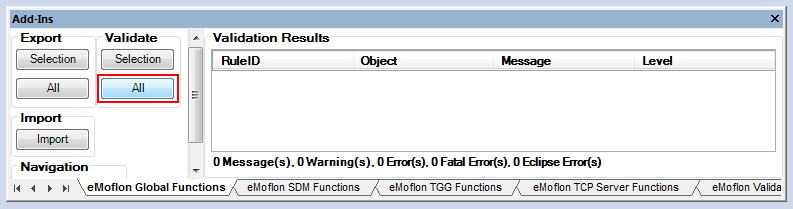
\includegraphics[width=\textwidth]{ea_importValidationWindow}
  \caption{No validation errors for \texttt{LeitnersLearningBox}}
  \label{ea:importValidationWindow}
\end{center}
\end{figure}

\vspace{0.5cm}

\item[$\blacktriangleright$] That's it! You now have the second metamodel for your transformation, and are ready to start specifying your TGG rules.

\jumpSingle{TGGSchema}

\end{itemize}


\newpage
\hypertarget{multiMOSL}{}
\subsection{Working with multple MOSL projects}
\texHeader

% Eclipse import instructions; all unconfirmed.
\begin{itemize}

\item[$\blacktriangleright$] Confirm your source metamodel \texttt{LeitnersLearningBox}, is in the current workspace prepared and right-click on
\texttt{MyWorkingSet}. Select \texttt{Import\ldots} from the context menu (Fig.~\ref{fig:eclipseContextImport}).

\vspace{0.25cm}

\begin{figure}[htbp]
\begin{center}
  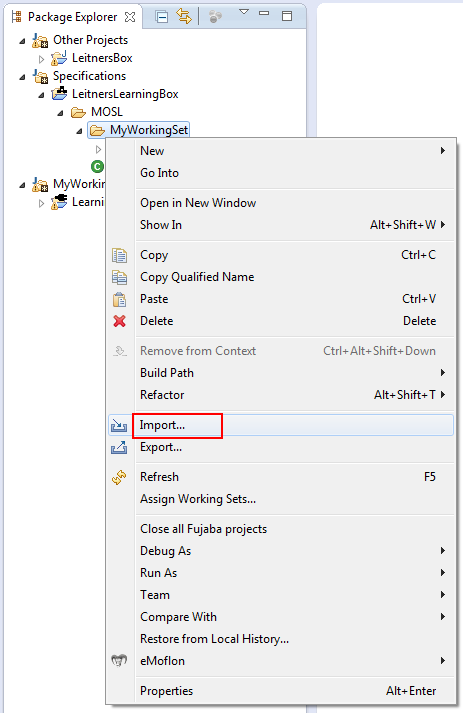
\includegraphics[width=0.6\textwidth]{eclipse_contextImport}
  \caption{caption}
  \label{fig:eclipseContextImport}
\end{center}
\end{figure}

\item[$\blacktriangleright$] In the first dialogue, set your import source by navigating to ``General/File System.'' This is the appropriate choice since
we want to import the entire directory structure of the target metamodel, not a pre existing project.

\item[$\blacktriangleright$] Press \texttt{Browse\ldots} and navigate to the folder where you extracted the contents of the \texttt{Part4.zip} download file
which included this document (Fig.~\ref{fig:importFileSys}). Press \texttt{Select All} to ensure you're importing all the necessary MOSL files for your TGG
target metamodel. Affirm and close the dialogue by pressing \texttt{Finish}.

\newpage

\begin{figure}[htbp]
\begin{center}
  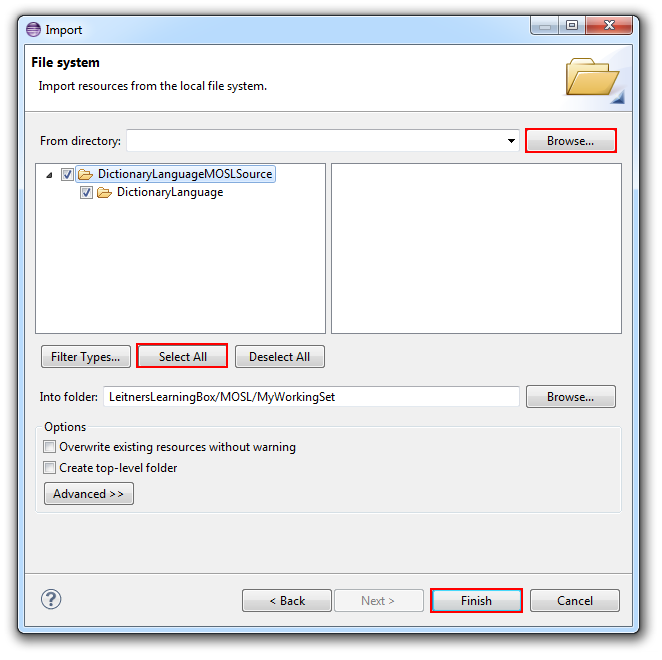
\includegraphics[width=0.8\textwidth]{eclipse_importDialogue}
  \caption{caption}
  \label{fig:importFileSys}
\end{center}
\end{figure}

\item[$\blacktriangleright$] With your project now loaded, navigate to ``Build (Without Cleaning)'' on the toolbar to build both metamodels. Confirm with
Fig.~\ref{fig:bothmetamodelstructures} that your MOSL directory is now populated with both metamodels, and notice that a second \texttt{Dictionary\-Language}
folder appeared under the same node as the \texttt{LearningBoxLanguage} repository project. If you expand this folder, you'll be able to see that it has
similar generated code for the imported metamodel.

\begin{figure}[htbp]
\begin{center}
  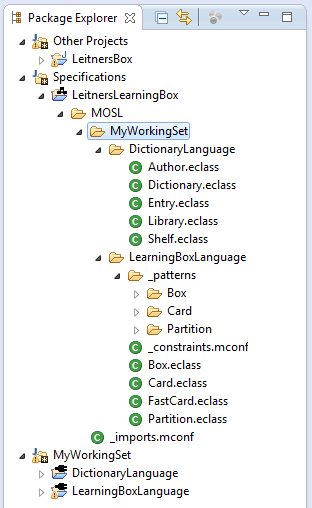
\includegraphics[width=0.5\textwidth]{eclipse_metamodelStructures}
  \caption{Fully loaded dual-metamodel structure}
  \label{fig:bothmetamodelstructures}
\end{center}
\end{figure}

\item[$\blacktriangleright$] Great work -- You're now ready to start using your metamodels in a TGG transformation! If you've just joined us and are interested
in the eMoflon project structure, or curious as to how Java code is generated, we invite you to read Section 4.2 from Part I. Otherwise, continue to the next section to begin
building your TGG Schema. 

\end{itemize}



% Declares ONE correspondence type: BoxToDictionary
\newpage
\hypertarget{TGGSchema}{}
\section{Creating your TGG schema}
\genHeader

Now that the necessary source and target metamodels are in the same workspace, there are several different ways to begin specifying a TGG. We're going to begin
with modeling the correspondence component of the triple language. This correspondence, or \emph{link metamodel},\define{Link \\ Metamodel} specifies
\emph{correspondence types},\define{Correspondence Types} which will be used to connect specific elements of the source and target metamodels. These
correspondence elements can also be thought of as \emph{traceability links}.

While the link metamodel is technically a standard metamodel, eMolfon uses a slightly different naming convention and concrete syntax to represent it. The
overall\define{TGG Schema} metamodel triple consisting of the relevant parts of the source, link, and target metamodels is called a \emph{TGG schema}.

A TGG schema can be viewed as the (metamodel) triple to which all \emph{new} triples must conform. In less technical lingo, it gives an abstract view on the
relationships (correspondence) between two metamodels or domains. A domain expert should be able to understand why certain connected elements are related,
irrespective of how the relationship is actually established by TGG rules, just by looking at the TGG schema. 

In our example schema, we will create a link between our source \texttt{Box} and target \texttt{Dictionary} to express that these two container elements are
related.

\jumpDual{schema vis}{schema tex}

\newpage
\hypertarget{schema vis}{}
\subsection{Visual Schema}
\visHeader

\begin{itemize}

\item[$\blacktriangleright$] Open \texttt{LearningBox2Dictionary.eap} in EA, and add a new package to \texttt{MyWorkingSet} (your model root) with
\texttt{Learning\-Box\-To\-Dictionary\-Integration} as its name (Fig.~\ref{fig:intgPackage}). 

\vspace{0.5cm}

\begin{figure}[htbp]
\begin{center}
  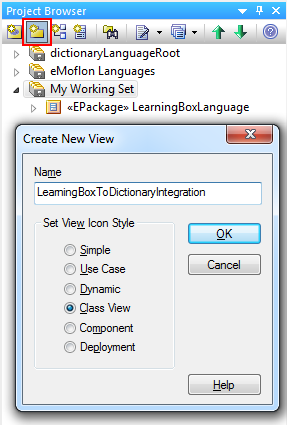
\includegraphics[width=0.4\textwidth]{ea_integrationPackage}
  \caption{Create a new package}  
  \label{fig:intgPackage}
\end{center}
\end{figure}


\item[$\blacktriangleright$] Create a diagram in the new package, selecting \texttt{TGGSchema} as diagram type (Fig.~\ref{fig:tgg_diagram_type}). The diagram
type indicates to EA that the new package is a TGG Project.

\vspace{0.5cm}

\begin{figure}[htbp]
\begin{center}
  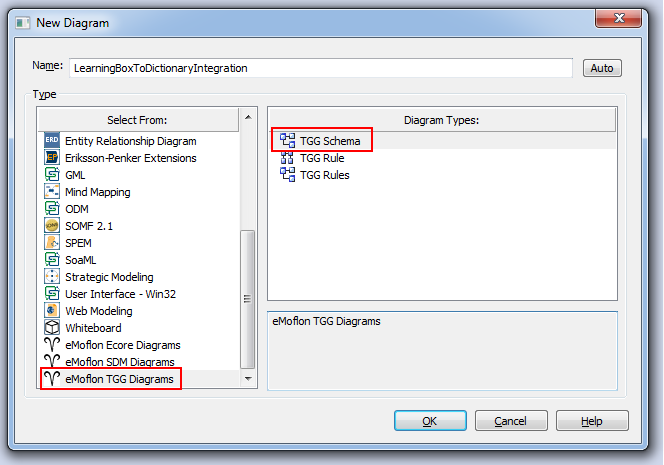
\includegraphics[width=0.9\textwidth]{ea_newTGGSchema}
  \caption{Choose \texttt{TGGSchema} as your diagram type}  
  \label{fig:tgg_diagram_type}
\end{center}
\end{figure}

\item[$\blacktriangleright$] After choosing \texttt{TGGSchema} as diagram type, a new dialogue should pop up asking you for the source and target projects of your TGG project. 
Choose \texttt{Learning\-Box\-Language} as source and \texttt{Dictionary\-Language} as target project and affirm with \texttt{OK} (Fig.~\ref{fig:select_source_target}).

\vspace{0.5cm}

\begin{figure}[htbp]
\begin{center}
  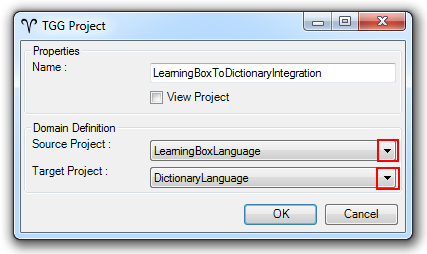
\includegraphics[width=0.55\textwidth]{ea_TGGSourceTarget}
  \caption{Select source and target projects for the TGG project}  
  \label{fig:select_source_target}
\end{center}
\end{figure}

\item[$\blacktriangleright$] The structure of your TGG project should now resemble Fig.~\ref{fig:new_tgg_project}. Please note that a subpackage \texttt{Rules}
and an underlying diagram with the same name are also generated.

\begin{figure}[htbp]
\begin{center}
  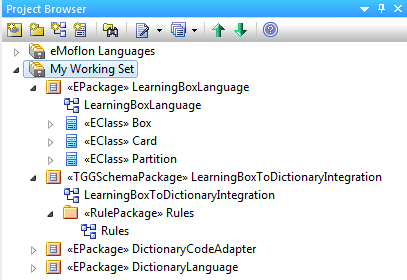
\includegraphics[width=0.5\textwidth]{ea_browserPostDiagram}
  \caption{Initial structure of a new TGG project}  
  \label{fig:new_tgg_project}
\end{center}
\end{figure}
\end{itemize}
\clearpage

Now it's time to insert classes from our source and target projects into our TGG project and declare our first \emph{correspondence type} between them.
The classes \texttt{Box} and \texttt{Dictionary} are to be related to each other.

\begin{itemize}
\item[$\blacktriangleright$] Hold \texttt{ctrl}, then drag-and-drop the \texttt{Box} class from \texttt{Learning\-Box\-Language} into the newly created TGG
schema diagram, which should have automatically opened in the editor when you made it. Ensure that the class is pasted \texttt{as a simple link} into the
diagram (Fig.)

\begin{figure}[htbp]
\begin{center}
  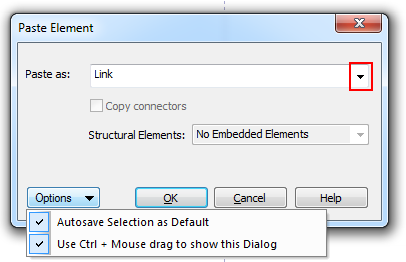
\includegraphics[width=0.6\textwidth]{ea_TGGDragDrop}
  \caption{Copying an element as a simple link} 
  \label{fig:TGGdragDrop}
\end{center}
\end{figure}

\item[$\blacktriangleright$] If you selected the \texttt{Autosave Selection as default} option during the previous drag and drop, you no longer need to hold
\texttt{ctrl} to bring the \texttt{Dictionary} class from \texttt{Dictionary\-Language} into the TGG schema.
\end{itemize}

With a class from both source and target projects, we can now create a correspondence type between them.

\begin{itemize}
\item[$\blacktriangleright$] Quick-link from \texttt{Box} to \texttt{Dictionary} and select \texttt{Create TGG Corres\-pon\-dence Type} as depicted in
Fig.~\ref{fig:create_correspondence}.
\end{itemize}

\begin{figure}[htbp]
\begin{center}
  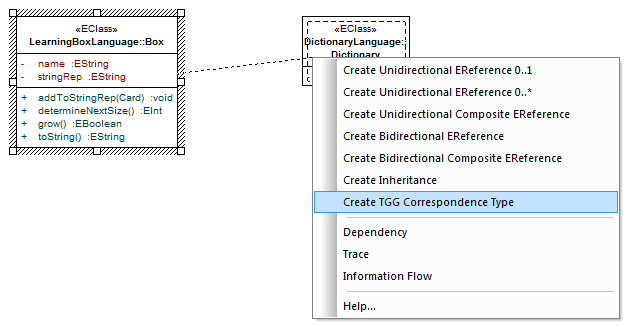
\includegraphics[width=\textwidth]{ea_TGGCorrespType}
  \caption{Creating a TGG correspondence type} 
  \label{fig:create_correspondence}
\end{center}
\end{figure}

A hexagon-shaped correspondence type named \texttt{BoxToDiction\-ary}, and references to each source and target element should have been generated.
You can rename the type as you wish, but please leave the references as they are (multiplicity and naming conventions are satisfied automatically).

To finish our TGG schema, declare a second correspondence type in the same file between \texttt{Card} and \texttt{Entry}. You'll notice that the
reference between \texttt{Dictionary} and \texttt{Entry} was automatically created! Your completed TGG Schema should resemble
Fig.~\ref{fig:complete_tgg_schema}.

\begin{figure}[htbp]
\begin{center}
  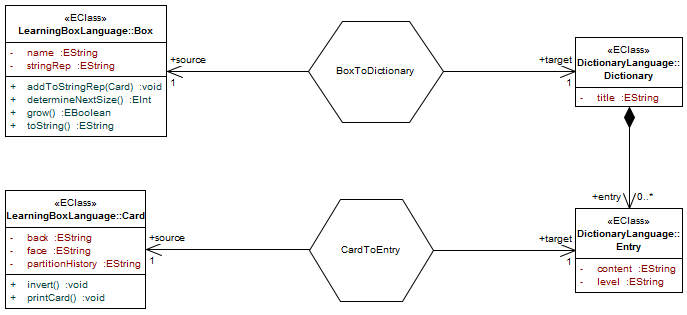
\includegraphics[width=\textwidth]{ea_completeTGGSchema}
  \caption{Complete TGG schema for our example}
  \label{fig:complete_tgg_schema}
\end{center}
\end{figure}



\newpage
\hypertarget{schema tex}{}
\subsection{Textual TGG Schema}
\texHeader

\begin{itemize}

\item[$\blacktriangleright$] Within the learning box metamodel folder, right-click on \texttt{MyWorkingSet}, and navigate to ``New / TGG''
(Fig.~\ref{eclipse:contextTGG}).

\vspace{0.5cm}

\begin{figure}[htbp]
\begin{center}
  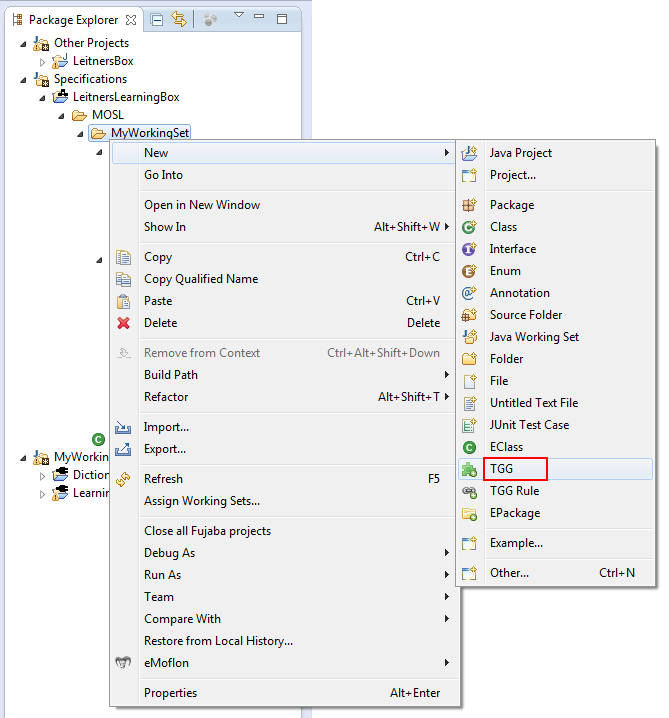
\includegraphics[width=0.8\textwidth]{eclipse_contextNewTGG}
  \caption{Creating a new TGG schema}
  \label{eclipse:contextTGG}
\end{center}
\end{figure}

\item[$\blacktriangleright$] Name the TGG \texttt{LearningBoxToDictionaryIntegration}, setting the source as \texttt{LearningBoxLanguage}, and target as
\texttt{DictionaryLanguage} (Fig.~\ref{eclipse:newTGG}).

\vspace{0.5cm}

\item[$\blacktriangleright$] A new TGG \texttt{schema} file should now be active in the editor! This is the \emph{TGG Schema} which declares each
\emph{correspondence type} as an \texttt{integration class}. Press \texttt{ctrl + space bar} and use the auto completion to generate a new integration class.

\newpage

\begin{figure}[htbp]
\begin{center}
  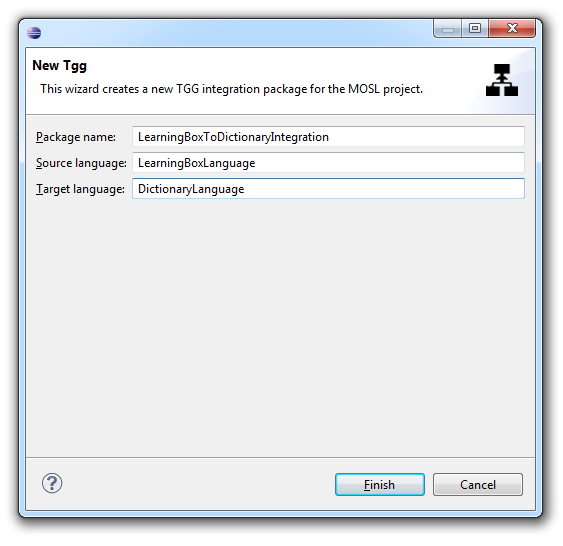
\includegraphics[width=0.8\textwidth]{eclipse_newTGG}
  \caption{Setting your \texttt{source} and \texttt{target} metamodels}
  \label{eclipse:newTGG}
\end{center}
\end{figure}

\item[$\blacktriangleright$] Note that when using a template, you can press \texttt{tab} to cycle through each element. Name the class
\texttt{BoxToDictionary}, and list the source as \texttt{Box} and target as \texttt{Dictionary} (Fig.~\ref{eclipse:firstCorrType}). 

\begin{figure}[htbp]
\begin{center}
  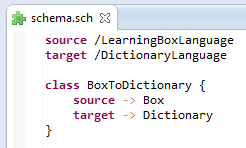
\includegraphics[width=0.4\textwidth]{eclipse_schemaFirstClass}
  \caption{Creating a correspondence type}
  \label{eclipse:firstCorrType}
\end{center}
\end{figure}

\item[$\blacktriangleright$] Believe it or not, that's all you need for your first correspondence type! Your schema is now complete with connections to your
\texttt{source} and \texttt{target} metamodels via a \emph{link} metamodel. To see the equivalent structure in the visual syntax, check out
Fig.~\ref{ea:firstCorrType} from the previous section.

\end{itemize}



% Develops BoxToDictionaryRule, CardToEntryRule, Builds (three repo projects), then explains the custom attribute constraint
\newpage
\hypertarget{sec:Rules}{}
\section{Specifying TGG rules}
\genHeader

With our correspondence type defined in the TGG schema, we can now specify a set of \emph{TGG rules} to describe a language of graph
triples.

As discussed in Section~\ref{sec:nutshell}, a TGG rule is quite similar to a SDM story pattern, following a \emph{precondition, postcondition}
format. This means we'll need to state:

\begin{itemize}

\item What must be matched (i.e., under which conditions can a rule be applied; `black' elements)

\item What is to be created when the rule is applied (i.e., which objects and links must exist upon exit; `green' elements)

\end{itemize}

\vspace{0.5cm}

Note that the rules of a TGG only describe the simultaneous \emph{build-up} of source, correspondence, and target models. Unlike SDMs, they do not delete or
modify any existing elements. In other words, TGG rules are \emph{monotonic}.\define{Monotonic}This might seem surprising at first, and you might even think
this is a terrible restriction. The intention is that a TGG should only specify a consistency relation, and \emph{not} the forward and backward transformations
directly, which are derived automatically. In the end, modifications are not necessary on this level but can, of course, be induced in certain
operationalizations of the TGG.

Let's quickly think about what rules we need in order to successfully transform a learning box into a dictionary. We need to first take care of the \texttt{box}
and \texttt{dictionary} structures, where \texttt{box} will need at least one \texttt{partition} to manipulate its \texttt{card}s. If more than one is created,
those partitions will need to have appropriate \texttt{next} and \texttt{previous} links. Conversely, given that \texttt{Dictionary} is unsorted, there are no
counterparts for partitions. A second rule will be needed to transform \texttt{card}s into \texttt{entries}. More precisely, a one-to-one correspondence must be
established (i.e., one \texttt{card} implies one \texttt{entry}), with suitable
concatenation or splitting of the contents (based on the transformation direction), and some mechanism to assign difficulty levels to each \texttt{entry} or initial position of each \texttt{card}.

\jumpDual{rules vis}{rules tex}

\newpage
\hypertarget{rules vis}{}
\subsection{BoxToDictionaryRule}
\genHeader

\begin{stepbystep}

\item Select the created subpackage \texttt{src/org.moflon.tgg.mosl.rules} (Step 1 in \Cref{ea:create_tgg_rule}) and click on the wizard \menuPath{Create new TGG rule} (\eMoflonCreateTGGRuleIcon, Step~2).
In the dialogue that pops up, enter \texttt{BoxToDictionaryRule} as the name of the TGG rule to be created.
Open the newly created file.

\begin{figure}[htbp]
\begin{center}
  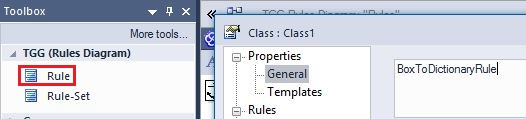
\includegraphics[width=0.8\textwidth]{../../org.moflon.doc.handbook.04_tripleGraphTransformations/4_rules/visRImages/ea_TGGNewRule.jpg}
  \caption{Creating a TGG rule}
  \label{ea:create_tgg_rule}
\end{center}
\end{figure}

\begin{figure}[htbp]
\begin{center}
  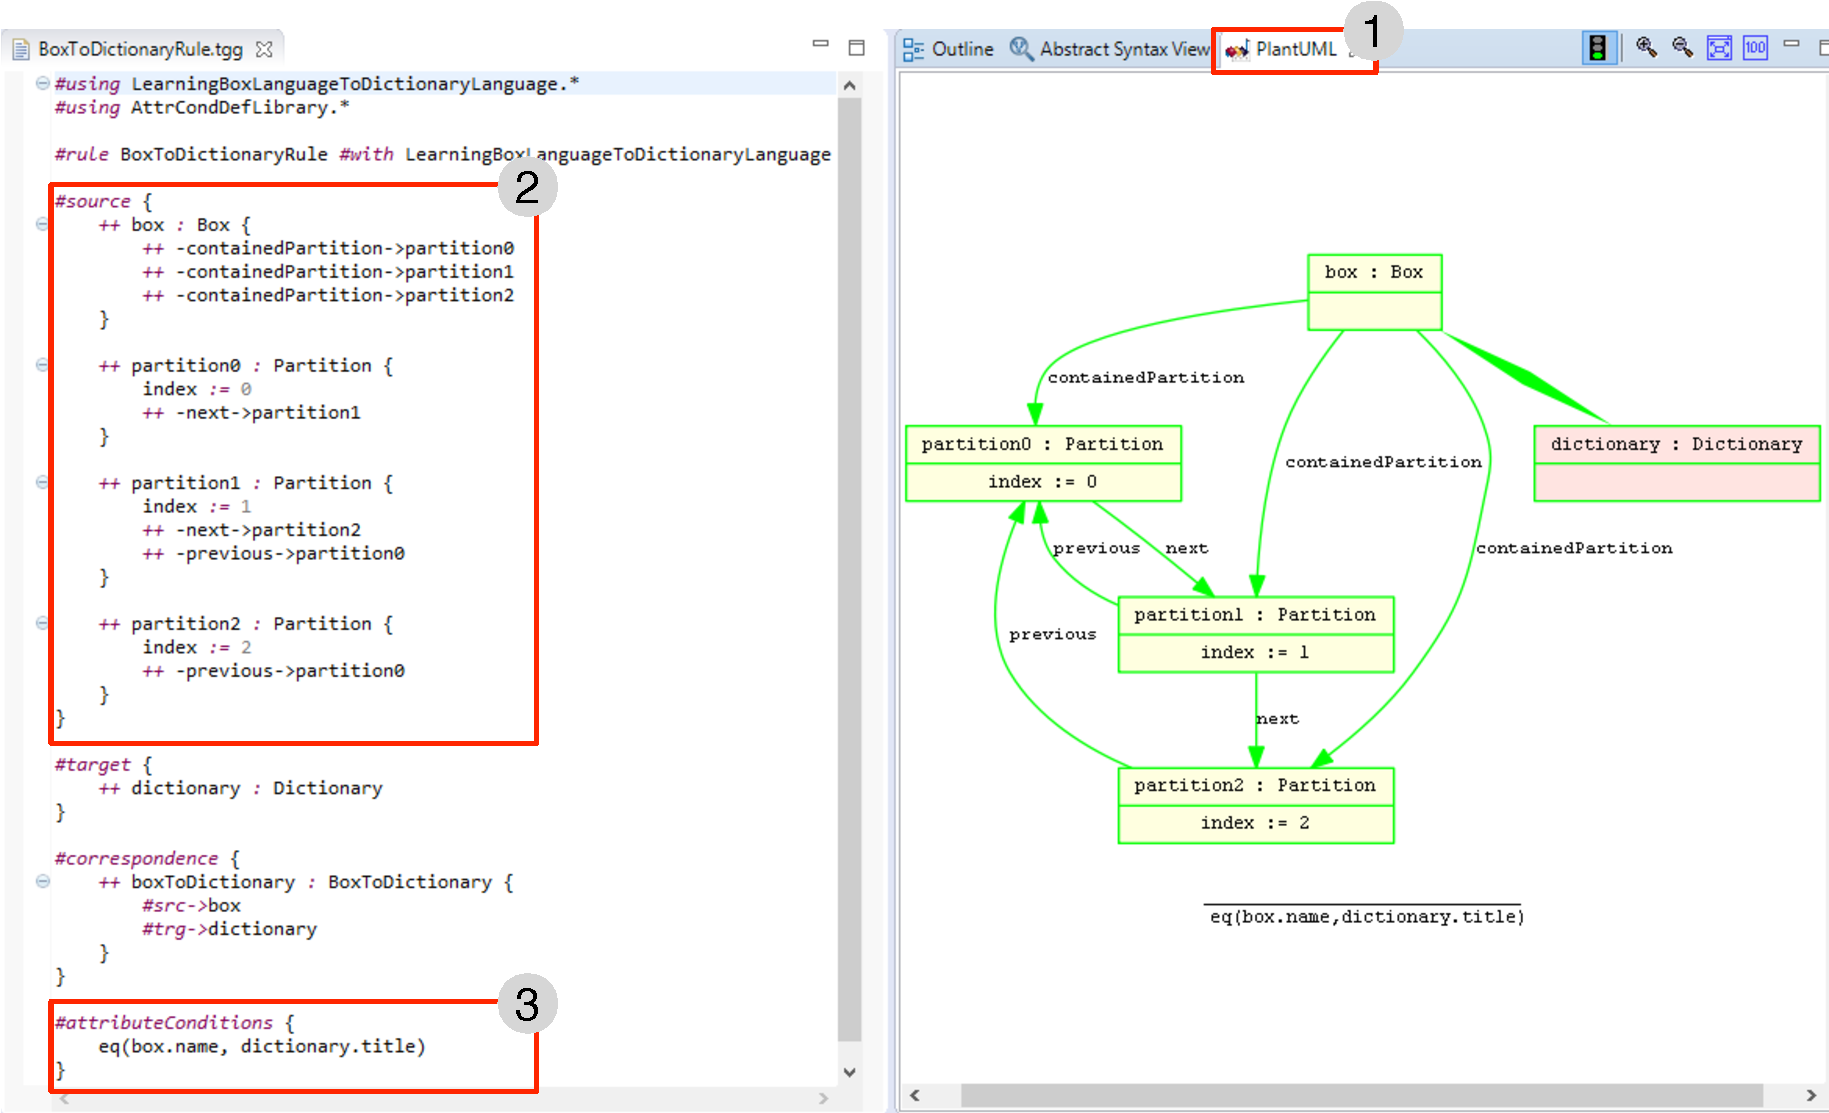
\includegraphics[angle=90,width=\textwidth]{../../org.moflon.doc.handbook.04_tripleGraphTransformations/4_rules/visRImages/ea_BoxToDictionaryRuleComplete.pdf}
  \caption{Complete TGG rule diagram for \texttt{BoxToDictionaryRule}}
  \label{ea:boxtodictionaryrule_complete}
  \end{center}
\end{figure}

\item  Ensure that you open the \texttt{PlantUML} view (Step 1 in \Cref{ea:boxtodictionaryrule_complete}) as it provides a helpful visualisation of the current TGG rule opened in the editor.
To prevent slowing you down, the view is only updated when you save \emph{and} change your cursor position.

Elements in the source domain have a yellow background, while target elements have a peach background.
Basic UML object diagram syntax is used, extended with colours to represent created elements (green outline) and context elements (black outline).

\texttt{BoxToDictionaryRule} is a so-called \emph{island rule} and only has created elements.
For presentation purposes, correspondence links are abstracted from in the visualisation and are depicted as bands (\eg, between \texttt{box} and \texttt{dictionary}).
The rule we want to specify creates a minimal dictionary (just a \texttt{Dictionary} node), and a minimal box, which is a bit more interesting as it consists already of three correctly connected partitions.
Any structure less than this is not a valid learning box.

\item The textual syntax we use is pretty straightforward:  every domain has a scope (\moslTggCode{\#source}, \moslTggCode{\#target}, and \moslTggCode{\#correspondence}), and there is a final scope for so called attribute conditions, which express how attribute values relate to each other.
The domain scopes contain again scopes for each \emph{object variable} in the rule (e.g., \texttt{box}) and these scopes then contain outgoing \emph{link variables} (\eg, \moslTggCode{-contained\-Partition->}), as well as inline attribute conditions (\eg, \moslTggCode{index := 0}).
Go ahead and specify the source scope as depicted in Step 2 of \Cref{ea:boxtodictionaryrule_complete}.
Notice how the \moslTggCode{++} operator is used to mark object and link variables as created or context variables.
Try removing and adding it and see how the visualisation changes.  
As always, let the editor help you by pressing \shortcut{Ctrl+Space} as often as possible.

\item Specify the \moslTggCode{#correspondence} and \moslTggCode{#target} scopes accordingly and make sure your rule (and its visualisation) closely resembles \Cref{ea:boxtodictionaryrule_complete}.

\item To complete our first rule, specify an attribute condition (inside the \moslTggCode{#attributeConditions} scope) to declare that the name of the box and the title of the dictionary are always to be equal.
As depicted in Step 3 \Cref{ea:boxtodictionaryrule_complete}, this can be accomplished using an \texttt{eq} condition.
We provide a standard library of such attribute conditions (press \shortcut{F3} on the constraint to jump to the library file), but it is also possible to extend this library with your own attribute conditions.
We'll see how to do this in a moment.
\end{stepbystep}

Fantastic work! The first rule of our transformation is complete! 
If you are in hurry, you could jump ahead and proceed directly to \Cref{sect:TGGs_in_Action}: TGGs in Action. 
There you can transform a box to a dictionary and vice-versa, but please be aware that your specified TGG (with just one rule) will only be able to cope with completely empty boxes and dictionaries. 
Handling additional elements (i.e., cards in the learning box and entries in the dictionary) requires a second rule.
We intend to specify this next.

\subsection{CardToEntryRule}

Our next goal is to be able to handle \texttt{Card} and \texttt{Entry} elements. 
The new thing here is that it will require a pre-condition -- you should not be able to transform these child elements (cards and entries) unless certain structural conditions (their parents exist and are related) are met. 
In other words, we need a rule that demands an already existing \texttt{box} and \texttt{dictionary}. 
It will need to combine `black' and `green' variables! 

\begin{stepbystep}

\item As we'll be connecting cards and entries, we need a new correspondence type.
Open the TGG schema (\filename{Schema.tgg}) and add a new correspondence type \moslTggCode{CardToEntry} connecting a \texttt{Card} (\moslTggCode{#src}) and an \texttt{Entry} (\moslTggCode{#trg}).

\item Create a new TGG rule with \texttt{CardToEntryRule} its name, and specify the rule as depicted in \Cref{ea:cardtoentry_1}.
\end{stepbystep}

Your diagram should now resemble \Cref{ea:cardtoentry_1}. 
We're not done yet though, we still need to handle attributes!
To understand why, consider the current rule and ask yourself  \emph{which} partition is meant.
Exactly!  This is currently not specified, so \emph{any} partition can be taken when applying the rule.
eMoflon would actually collect all applicable rules (one for every partition) and consult a configuration component to decide which rules should be taken.
The default component just chooses randomly, but you could override this and, \eg, pop up a dialogue asking the user which partition to use.
Although this could be an interesting solution, we'll see how to fully specify things using extra attribute conditions.

\begin{figure}[htbp]
  \begin{center}
    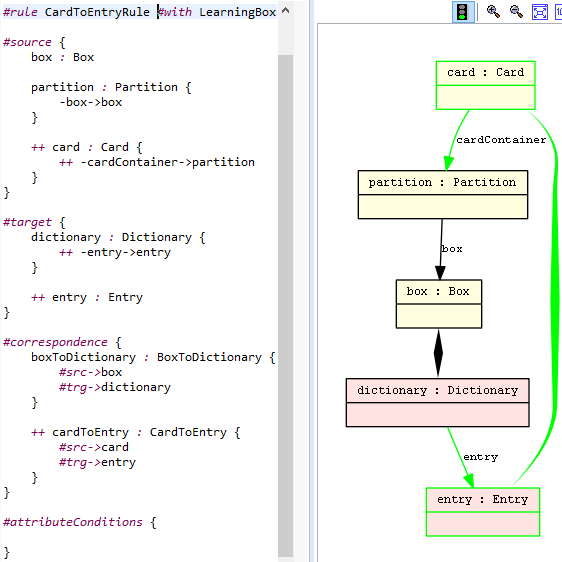
\includegraphics[width=\textwidth]{../../org.moflon.doc.handbook.04_tripleGraphTransformations/4_rules/visRImages/ea_cardToEntryRule.PNG}
    \caption{\texttt{CardToEntryRule} without attribute manipulation}
    \label{ea:cardtoentry_1}
  \end{center}
\end{figure}

On the way to handling all attributes, let's first start with the relatively easy case of specifying how every \moslTggCode{entry.content}, \moslTggCode{card.back}, and \moslTggCode{card.face} relate to each other.
We should probably combine the front and back of each card as a single content attribute of an entry and, in the opposite direction, split the content into \texttt{card.back} and \texttt{card.face}.

So let's define \moslTggCode{entry.content} as: \moslTggCode{<word>:<meaning>}. 
Therefore, \moslTggCode{card.back} should be \moslTggCode{Question:<word>} and similarly, \moslTggCode{card.face} should be \moslTggCode{Answer:<meaning>}. 

\begin{stepbystep}
\item Luckily, we have two library attribute conditions, \texttt{addPrefix} and \texttt{concat} to help us with this.
Add the following to the \moslTggCode{#attributeConditions} scope of your rule:

\moslTggCode{addPrefix("Question ", word, card.back)}\\  
\moslTggCode{addPrefix("Answer ", meaning, card.face)}\\
\moslTggCode{concat(":", word, meaning, entry.content)}

\moslTggCode{Question} and \moslTggCode{Answer} are EString literals, \moslTggCode{word} and
\moslTggCode{meaning} are local variables, and \moslTggCode{card.face}, \moslTggCode{card.back}, and \moslTggCode{entry.content} are attribute expressions.

\item Our final task is now to specify where a new \moslTggCode{card} (when transformed from an \moslTggCode{entry}) should be placed.  
We purposefully created three partitions to match the three difficulty levels, but if you check the available library constraints, there is nothing that can directly implement this specific kind of mapping. 
We will therefore need to create our own attribute condition to handle this.

\item Open the TGG schema (\filename{Schema.tgg}), and define a new attribute condition in the \moslTggCode{#attributeConditions} scope. 
Name it \moslTggCode{indexToLevel}, and enter the values given in \Cref{ea:create_new_constraint}.

\begin{figure}[htbp]
\begin{center}
  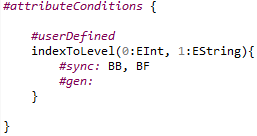
\includegraphics[width=0.45\textwidth]{../../org.moflon.doc.handbook.04_tripleGraphTransformations/4_rules/visRImages/ea_uniqueConstraint.PNG}
  \caption{Specifying the new attribute condition \moslTggCode{indexToLevel}}
  \label{ea:create_new_constraint}
\end{center}
\end{figure}
\FloatBarrier

\item Please note that this is just a \emph{specification} of a custom attribute condition -- we still need to actually implement it in Java! 
As we're so close to finishing this TGG rule, however, let's complete it first before we work out the exact meaning of the mysterious adornments (those funny \texttt{BB}, \texttt{BF}, \dots) and parameters (\texttt{0:EInt} and \texttt{1:EString}) of the attribute condition. 
For now, just make sure you enter the exact values in \Cref{ea:create_new_constraint}. 

\item We can now use this new attribute condition \moslTggCode{indexToLevel} just like any of the library attribute conditions.
Add the following code to the \moslTggCode{#attributeConditions} scope of the \texttt{CardToEntryRule} to express that the relationship between the index of the partition containing the new card, and the level of the new entry, is defined by our new attribute condition:

\moslTggCode{indexToLevel(partition.index, entry.level)}
\end{stepbystep}

If everything has been done correctly up to this point, your project should save and build.
The generated code will have some compilation errors (Step 1 in Fig.~\ref{eclipse:tggGenerated}) as Eclipse does not know where to access the generated code for the imported source and target ecore files (these could also be supplied from jars or installed plugins).
In our case the generated code is in the respective source and target projects so let's communicate this to Eclipse.

\begin{stepbystep}

\item Open the \texttt{MANIFEST.MF} file (Step 2 in Fig.~\ref{eclipse:tggGenerated}) and choose the \texttt{De\-pen\-den\-cies} tab (Step 3).

\item Choose both source and target projects (\texttt{DictionaryLanguage}, \texttt{Learning\-Box\-Language}, Step 4) as dependencies and click \texttt{OK}.
All compilations errors should now be resolved.
\end{stepbystep}

\begin{figure}[htb]
\begin{center}
  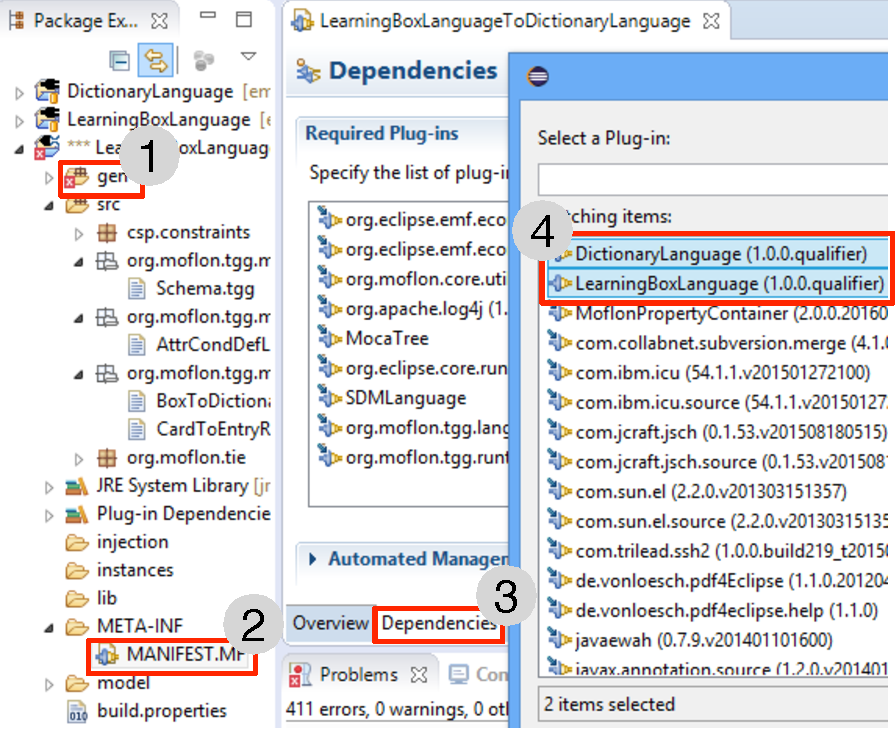
\includegraphics[width=0.8\textwidth]{../../org.moflon.doc.handbook.04_tripleGraphTransformations/4_rules/eclipse_generatedTGG.pdf}
  \caption{Add source and target projects as dependencies}
  \label{eclipse:tggGenerated}
\end{center}
\end{figure}

Great work! All that's left to do is implement the \texttt{indexToLevel} constraint, and give your transformation a test run.


\newpage
\hypertarget{rules tex}{}
\subsection{Tex Rules}
\texHeader

Some sort of content so that we don't start right away with a subsection. It should be two lines long.

\subsection{BoxToDictionaryRule}

\begin{itemize}

\item[$\blacktriangleright$] You may have noticed that a \texttt{Rules} folder was created and included in the TGG package when you first created it. Create
your first one by right-clicking on the folder and navigating to ``New/TGG Rule.'' Name it \texttt{BoxToDictionaryRule}, and confirm the file opens in the
editor window.

\item[$\blacktriangleright$] You'll notice that the rule is clearly separated into its three areas -- \texttt{source}, \texttt{correspondence}, and
\texttt{target}. There is a fourth scope, \texttt{constraints}, is where you can can list CSP constraints which manipulate attributes based on the
transformation direction. 

\item[$\blacktriangleright$] Lets first establish the \texttt{target} and \texttt{source} structures. Given that this is the first rule to be applied in a
transformation, we can assume there is no context to work with, so each of our objects will need to be set to `green' (create). In the \texttt{source} scope,
create a \texttt{box} of type \texttt{Box}. Similarily, in the \texttt{target} scope, create a \texttt{dictionary} of type \texttt{Dictionary}. Your rule
should now resemble Fig.~\ref{fig:textSourceRule}.

\vspace{0.5cm}

\begin{figure}[htbp]
\begin{center}
  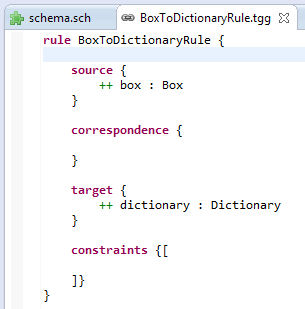
\includegraphics[width=0.5\textwidth]{eclipse_boxToDictionary_start}
  \caption{start BoxToDictionary}
  \label{fig:textSourceRule}
\end{center}
\end{figure}

\item[$\blacktriangleright$] Now we can create our first TGG Correspondence link! In the \texttt{correspondence} scope, enter 
\syntax{++ box <- boxToDictionary : BoxToDictionary -> dictionary}
Note that the structure of this statement creates \emph{one} link, named \texttt{boxToDictionary}, of correspondence type \texttt{BoxToDictionary} which was
delcared in the schema.

\end{itemize}

If this rule were to be run at this point, as-is, it would be actually successful by creating a single \texttt{Box} and \texttt{Dictionary}! Besides the
correspondence link however, these items have nothing in common. Let's try connecting the \texttt{name} of \texttt{box} to the \texttt{title} of \texttt{dictionary} with an
\emph{attribute constraint}. In TGG rules, attribute constraints provide a bidirectional and high level solution for attribute manipulations. In addition to the
basic math constraints such as addition (add), subtraction (sub), divide, max, multiply, and smallerOrEqual, we have some preexisting string constraints
we can use in this application. These include stringToNumber, concat, addPrefix, addSuffix, and equals (eq).

\begin{itemize}

\item[$\blacktriangleright$] Therefore, under the \texttt{constraints} scope, write:
\syntax{eq(box.name, dictionary.title)}
Your rule should now resemble Fig.~\ref{fig:ruleBasic}.

\vspace{0.5cm}

\begin{figure}[htbp]
\begin{center}
  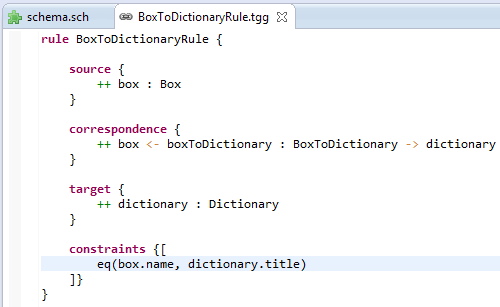
\includegraphics[width=0.8\textwidth]{eclipse_boxToDictionary_firstElements}
  \caption{first elements}
  \label{fig:ruleBasic}
\end{center}
\end{figure}

\end{itemize}

Switch back to \texttt{BoxToDictionaryRule}. What's missing from our rule? We have created the primary container structures for the \texttt{target} and
\texttt{source}, but \texttt{cards} cannot be stored directly in \texttt{box}! We therefore need to create some \texttt{partition} objects. 

\begin{itemize}

\item[$\blacktriangleright$] Given that there are three difficulty \texttt{level}s for each dictionary \texttt{entry}, create and complete \texttt{partition0},
\texttt{partition1}, and \texttt{partition2} with the appropriate \texttt{containedPartition}, \texttt{next} and \texttt{previous} link variables so that your
rule matches Fig.~\ref{fig:allReferences}.\footnote{Read the introduction to Part II to review the rules and motivation behind our LeitnersBox}

\end{itemize}

\begin{figure}[htbp]
\begin{center}
  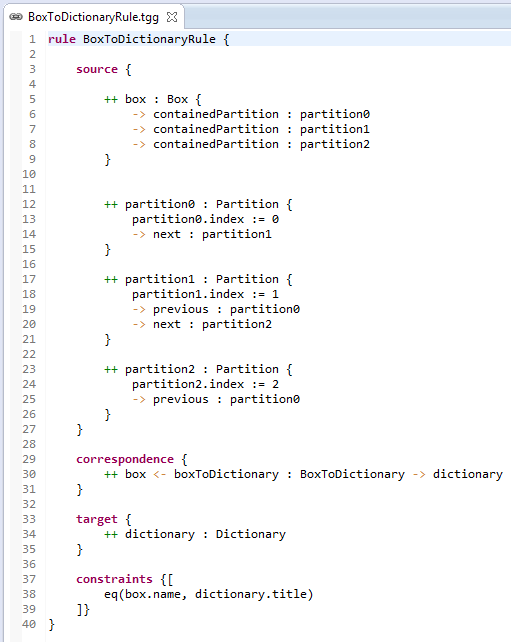
\includegraphics[width=0.8\textwidth]{eclipse_boxToDictionary_complete}
  \caption{First rule complete}
  \label{fig:allReferences}
\end{center}
\end{figure}


Great work! Your first TGG rule is complete! This rule is able to transform a \texttt{box} into a \texttt{dictionary} and vice-versa. Unfortunately, it will
only be able to handle completely \emph{empty} boxes and dictionaries -- you can see that we haven't provided additional handling for \texttt{Card} or
\texttt{Entry} items. If you're in a hurry, feel free to jump ahead to Section 4: TGGs in Action to execute this rule. Otherwise, the next rule we create will
integrate itself with \texttt{BoxToDictionaryRule} to take care of this.


% --------------- Card To Entry ------------------------------------------------------------------------------------------------------------------------
\subsection{CardToEntryRule}

\begin{itemize} 

\item[$\blacktriangleright$] Analogously to how you began the previous rule, return to the TGG schema and create a second \emph{Integration Class} called
\texttt{CardToEntry} with a \texttt{Card} source and \texttt{Entry} target. Your updated file should now resemble Fig.~\ref{fig:updatedSchema}.

\vspace{0.5cm}

\begin{figure}[htbp]
\begin{center}
  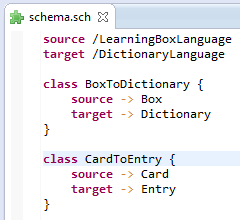
\includegraphics[width=0.4\textwidth]{eclipse_updatedSchema}
  \caption{udpated schema}
  \label{fig:updatedSchema}
\end{center}
\end{figure}

\item[$\blacktriangleright$] Right click on the \texttt{Rules} folder again, and create a \texttt{CardToEntryRule}.

\end{itemize}

One of the key differences between this rule and the last is that \texttt{CardToEntryRule} will only be invoked within a certain context i.e.,
this will only be used if a preexisting \texttt{partition} has \texttt{card} elements that need to be transformed into entires in an established
\texttt{dictionary}. In terms of MOSL, this means there will be both `black' and `green' elements.

\begin{itemize}

\item[$\blacktriangleright$] To begin, create three object variables in the \texttt{source} scope: \texttt{box}, \texttt{partition0}, and \texttt{card}. Which
ones are already known from the context? Which element still needs to be made? Your rule should come to resemble Fig.~\ref{fig:c2eRuleSource}.

\begin{figure}[htbp]
\begin{center}
  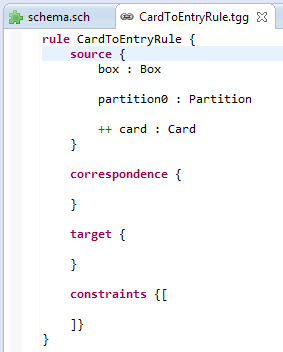
\includegraphics[width=0.45\textwidth]{eclipse_cardToEntry_sourceOVs}
  \caption{source filled}
  \label{fig:c2eRuleSource}
\end{center}
\end{figure}

\item[$\blacktriangleright$] In the \texttt{target} scope, we will know \texttt{dictionary} from the context, but will still need to create a new entry object
via \texttt{++ entry:Entry}.

\vspace{0.5cm}

\item[$\blacktriangleright$] Now we can complete the \texttt{correspondence}! Our contextual \texttt{box} and \texttt{dictionary} objects can be connected via
the same \texttt{boxToDictionary} link as declared in \texttt{BoxToDictionaryRule}, but a second link needs to be created between \texttt{card} and \texttt{entry}.
Use the correspondence type from the updated schema and write: \syntax{++ card <- cardToEntry : CardToEntry -> entry}

% \begin{figure}[htbp]
% \begin{center}
%   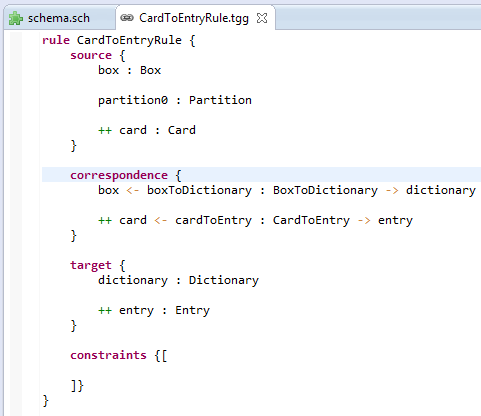
\includegraphics[width=0.8\textwidth]{eclipse_cardToEntry_correspondence}
%   \caption{correspondence}
%   \label{fig:c2etargetCorresp}
% \end{center}
% \end{figure}

\vspace{0.5cm}

\item[$\blacktriangleright$] Finally, let's make sure the transformation is able to access the \texttt{card} and \texttt{entry} attributes. Complete each
of your \texttt{box}, \texttt{partition0}, and \texttt{dictionary} object variable scopes until your rule matches Fig.~\ref{fig:c2eAllReferences}.\footnote{Don't
forget that eMoflon's type completion can help you establish references here; Press \texttt{ctrl + space bar} after writing \texttt{->} for a list of available
link variables from the relevant \texttt{eclass}.}

\newpage

\begin{figure}[htb]
\begin{center}
  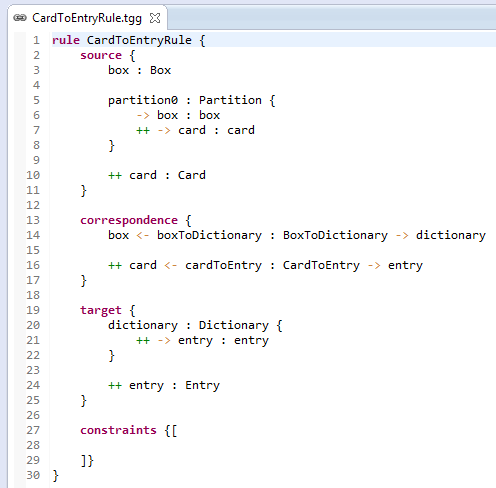
\includegraphics[width=0.8\textwidth]{eclipse_cardToEntry_objectVariables}
  \caption{all object variables}
  \label{fig:c2eAllReferences}
\end{center}
\end{figure}

\end{itemize}

Finally, let's establish the necessary \texttt{constraints} which can handle the relevant content attributes of \texttt{card} and \texttt{entry}. We'll need to
first decide on some common variables and syntax between \texttt{card.face}, \texttt{card.back}, and \texttt{entry.content} so that we can combine each side of
a \texttt{card} into one attribute, or split each \texttt{entry} into a question and answer. 

\begin{itemize}

\item[$\blacktriangleright$] Except perhaps on a piece of paper so you can keep track, let's define the syntax for \texttt{entry.content} as
\texttt{<word>:<meaning>}, \texttt{card.back} as \texttt{Question:<word>}, and \texttt{card.face} as \texttt{Answer:<meaning>}. 

\vspace{0.5cm}

\item[$\blacktriangleright$] Now, using the preexisting String attribute constraint types, edit your \texttt{constraint} scope until it resembles
Fig.~\ref{fig:contentConstraints}.

\begin{figure}[htbp]
\begin{center}
  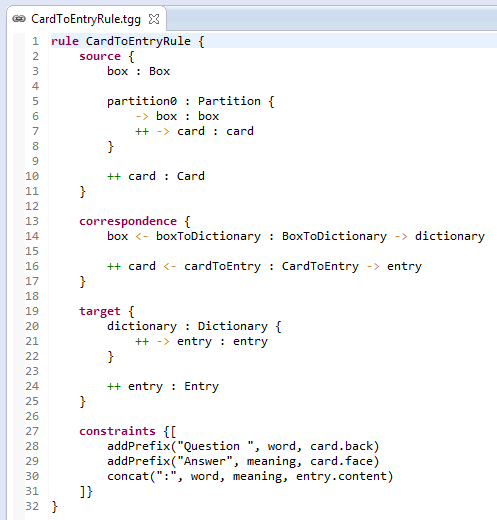
\includegraphics[width=0.8\textwidth]{eclipse_cardToEntry_firstConstraints}
  \caption{preexisting constraints}
  \label{fig:contentConstraints}
\end{center}
\end{figure}

\end{itemize}

\newpage

Let's add \emph{one} more constraint. Given that we have three partitions, and three difficulty levels for each \texttt{Entry}, why don't we have the
transformation assign a level based on whatever partition a \texttt{card} is found in? Hard cards, for example, are more likely to be found in the first
partition (due to being shifted backwards from wrong guesses).  As you can imagine, there is no constraint type currently existing in eMoflon to manage this --
we must create our own!

\begin{itemize}

\item[$\blacktriangleright$] Add the following declaration to the \texttt{constraint} scope: \syntax{indexToLevel[BB,BF,FB](EInt, EString)} We will discuss what
each of the options mean in a moment.

\vspace{0.5cm}

\item[$\blacktriangleright$] You can now invoke your rule with \texttt{indexToLevel(partition0.index, entry.level)} immediately below the declaration. Your
completed \texttt{CardToEntryRule} should now resemble Fig.~\ref{fig:c2eDone}.

\begin{figure}[htbp]
\begin{center}
  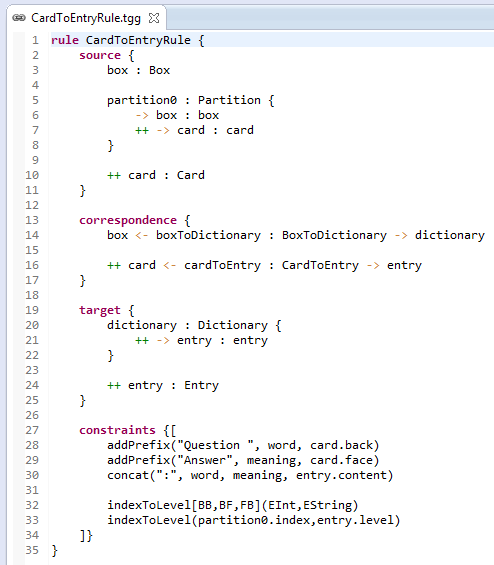
\includegraphics[width=0.9\textwidth]{eclipse_cardToEntry_complete}
  \caption{COMPLETED rule}
  \label{fig:c2eDone}
\end{center}
\end{figure}

\vspace{0.5cm}

\item[$\blacktriangleright$] Awesome work! If you haven't already, save the file and confirm the MOSL parser hasn't raised any errors. Press \texttt{``Build
(Without Cleaning)''}, and admire your TGG transformation rules. 

\vspace{0.5cm}

\item[$\blacktriangleright$] To see how \texttt{BoxToDictionaryRule} is implemented in the visual syntax, check out Fig.~\ref{fig:boxtodictionaryrule_complete}
from Section 4.1. The \texttt{CardToEntryRule} is depicted in Fig.~\ref{fig:cardtoentry_complete} in Section 4.2.

\end{itemize}


\hypertarget{subsec:IndexToLevel}{}
\subsection{Implementing IndexToLevel}
\genHeader

If everything has been done correctly up to this point, your project should save and build (hit the hammer symbol in the eMolfon task bar).
The generated code will have some compilation errors (Step 1 in \Cref{eclipse:tggGenerated}) as Eclipse does not know where to access the generated code for the imported source and target ecore files (these could also be supplied from jars or installed plugins).
In our case the generated code is in the respective source and target projects so let's communicate this to Eclipse.

\begin{enumerate}

\item[$\blacktriangleright$] Open the \texttt{MANIFEST.MF} file (Step 2 in \Cref{eclipse:tggGenerated}) and choose the \texttt{De\-pen\-den\-cies} tab (Step 3).

\item[$\blacktriangleright$] Choose both source and target projects (Step 4) as dependencies and click \texttt{OK}.
All compilations errors should now be resolved.
\end{enumerate}

\begin{figure}[htb]
\begin{center}
  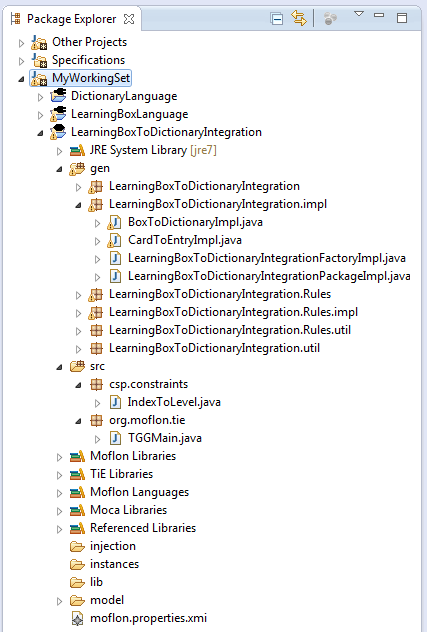
\includegraphics[width=0.8\textwidth]{eclipse_generatedTGG}
  \caption{Add source and target projects as dependencies}
  \label{eclipse:tggGenerated}
\end{center}
\end{figure}

Our TGG still isn't yet complete. 
While we've declared and actually used our custom \texttt{indexTolevel} attribute condition, we haven't actually implemented it yet. 
Let's quickly review the purpose of attribute conditions.

Just like patterns describing \emph{structural} correspondence, \emph{attribute conditions} can be automatically \emph{operationalized} as required, e.g., for a forward transformations. 
Even more interesting, a set of attribute conditions might have to be ordered in a specific way depending on the direction of the transformation.
Enforcing the conditions might involve checking existing attribute values, or setting these values appropriately.

For built-in \emph{library} attribute conditions such as \emph{eq}, \emph{addPrefix} and \emph{concat}, you do not need to worry about these details and can just focus
on expressing what should hold. 
Everything else is handled automatically.

In some cases however, a required attribute condition might be problem-specific, such as our \emph{indexToLevel}. 
There might not be any fitting combination of library attribute conditions to express the consistency condition, so a new attribute condition type must be declared and implemented.

There is a list of \emph{adornments} in the declaration which specify the cases for which the attribute condition can be operationalized. 
Each adornment consists of a \texttt{B} (bound) or \texttt{F} (free) variable setting for each argument of the attribute condition. 
This might sound a bit complex, but it's really quite simple, especially in the context of our example:

\begin{description}

\item[BB] indicates that the \texttt{partition.index} and \texttt{entry.level} are both \emph{bound}, i.e., they already have assigned values.
In this case, the \emph{operation} must check if the assigned values are valid and correct.

\item[BF] indicates that \texttt{partition.index} is \emph{bound} and \texttt{entry.level} is \emph{free}, i.e., the operation must determine and assign the correct value to \texttt{entry.level} using \texttt{partition.index}.

\item[FB] would indicate that \texttt{partition.index} is \emph{free} and \texttt{entry.level} is \emph{bound}, i.e., the operation must determine and assign the correct value to \texttt{parti\-tion.in\-dex} using \texttt{entry.level}.

\item[FF] would indicate that both \texttt{partition.index} and \texttt{entry.level} are \emph{free} and we have to somehow generate consistent values out of thin air.

\end{description}

As \texttt{partition} is a context element in the rule (the partition is always bound in whatever direction), \textbf{FF} and \textbf{FB} are irrelevant cases and we do not need to declare or implement what they mean.
For the record, note that adornments can be declared as either \texttt{\#gen} or \texttt{\#sync}.
The reason is that it might make sense to restrict some adornments (typically \textbf{FF} cases) to only when generating models.
Using \textbf{FF} cases for synchronisation might possibly makes sense, but most of the time it would be weird to generate random values during a forward or backward synchronisation.  

At compile time, the set of attribute conditions for every TGG rule is ``solved'' for each case by
operationalizing all constraints and determining a feasible sequence in which the operations can be executed, compatible to the declared adornments of each attribute condition. 
If the set of attribute conditions cannot be solved, an exception is thrown at compile time.

Now that we have a better understanding behind the construction of attribute conditions, let's implement \texttt{indexToLevel}.

\begin{itemize}
\item[$\blacktriangleright$] Locate and open \texttt{IndexToLevel.java} under ``src/csp.constraints'' in \texttt{LearningBoxToDictionaryIntegration}.

\item[$\blacktriangleright$] As you can see, some code has been generated in order to handle the current unimplemented state of \texttt{IndexToLevel}. 
Use the code depicted in \Cref{code:indexToLevel} to replace this default implementation.\footnote{Depending of course on your pdf viewer, copy and pasting this code should work.}

\begin{figure}[htb]
\begin{verbatim}
package csp.constraints;

import java.util.Arrays;
import java.util.List;
import org.moflon.tgg.language.csp.Variable;
import org.moflon.tgg.language.csp.impl.TGGConstraintImpl;

public class IndexToLevel extends TGGConstraintImpl {

    private static List<String> levels = 
      Arrays.asList(new String[] {"master","advanced","beginner"});

    public void solve(Variable var_0, Variable var_1) {
        int index = ((Integer) var_0.getValue()).intValue();
        int normalisedIndex = Math.min(Math.max(0, index), 2);
        String bindingStates = getBindingStates(var_0, var_1);
        
        switch (bindingStates) {
        case "BB":
            String level = (String) var_1.getValue();
            setSatisfied(levels.get(normalisedIndex).equals(level));
            break;
        case "BF":
            var_1.bindToValue(levels.get(normalisedIndex));
            setSatisfied(true);
            break;
        }}}
\end{verbatim}
  \caption{Implementation of our custom \texttt{IndexToLevel} constraint}
  \label{code:indexToLevel}
\end{figure}

\end{itemize}

To briefly explain, the \texttt{levels} list contains difficulty level at positions 0, 1, or 2 in the list, which correspond to our three partitions in the learning box. 
You'll notice that instead of setting ``master'' to 2, it has rather been set to match the first 0th partition. 
Unlike an \texttt{entry} in \texttt{dictionary}, the position of each \texttt{card} in \texttt{box} is \emph{not} based on difficulty, but simply how it has been moved as a result of the user's correct and incorrect guesses. 
Easy cards are more likely to be in the final partition (due to moving through the box quickly) while challenging cards are most likely to have been returned to (and currently to be at) the starting position, i.e., the 0th partition.

In the \texttt{solve} method, the index of the matched partition in the rule is first of all normalised (negative values do not make sense, and we handle all partitions  after partition 2 in the same way).
A switch statement is then used, based on whichever adornment is currently the case, to enforce or check the condition. 

For \texttt{BB} we check if the normalised index of the partition corresponds to the difficulty level of the card.
For \texttt{BF}, the normalised index is used to set the appropriate difficulty level of the card.

%%% Local Variables: 
%%% mode: latex
%%% TeX-master: "../src/TGG_mainFile"
%%% End: 



% Should run successfully on exclusively THREE partitions in BOX; creates one instance, runs it, renames it, ta daa
\newpage
\section{TGGs in action}
\genHeader
\label{sect:TGGs_in_Action}
In this section, we shall export our TGG, implement our new constraint, and get our integration running! The instructions for both syntaxes are virtually the
same, but keep a lookout for colored bullet arrows regarding syntax-specific commands

\vspace{0.5cm}

\begin{itemize}
\item[\color{RedOrange}$\blacktriangleright$] Export your metamodels and TGG from EA by choosing ``\texttt{Extensions/\-MOFLON::\-Ecore Addin\-/Export all to
Workspace}' and refresh your Eclipse metamodel project.

\vspace{0.5cm}

\item[\color{CornflowerBlue}$\blacktriangleright$] Go to the toolbar and press \texttt{Build (without cleaning)}, and make sure your metamodel project
refreshes.
\end{itemize}

\vspace{0.5cm}

If you have done everything right, code generation and compilation should terminate without error, and the structure of the \texttt{gen} folder in
\texttt{LearningBox\-To\-Dictionary\-Integration} should resemble Fig.~\ref{fig:gen_folder}.

\begin{figure}[htbp]
\begin{center}
  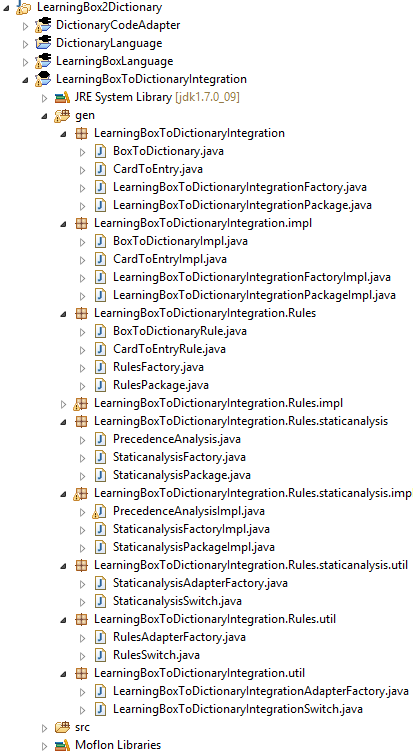
\includegraphics[width=0.8\textwidth]{tgg22}
  \caption{Integration project after code generation}
  \label{fig:gen_folder}
\end{center}
\end{figure}

\begin{itemize}

\vspace{0.5cm}
  
\item[$\blacktriangleright$] To implement the \texttt{IndexToLevel} constraint, locate and open the file \texttt{csp/IndexToLevel.java} under
  ``LearningBoxToDictionaryIntegration/src/'' 

\vspace{0.5cm}
  
\item[$\blacktriangleright$] Copy and paste the code provided in Fig.~\ref{fig:indexToLevel} into the file.

\end{itemize}

\begin{figure}[htbp]
\begin{center}
  % 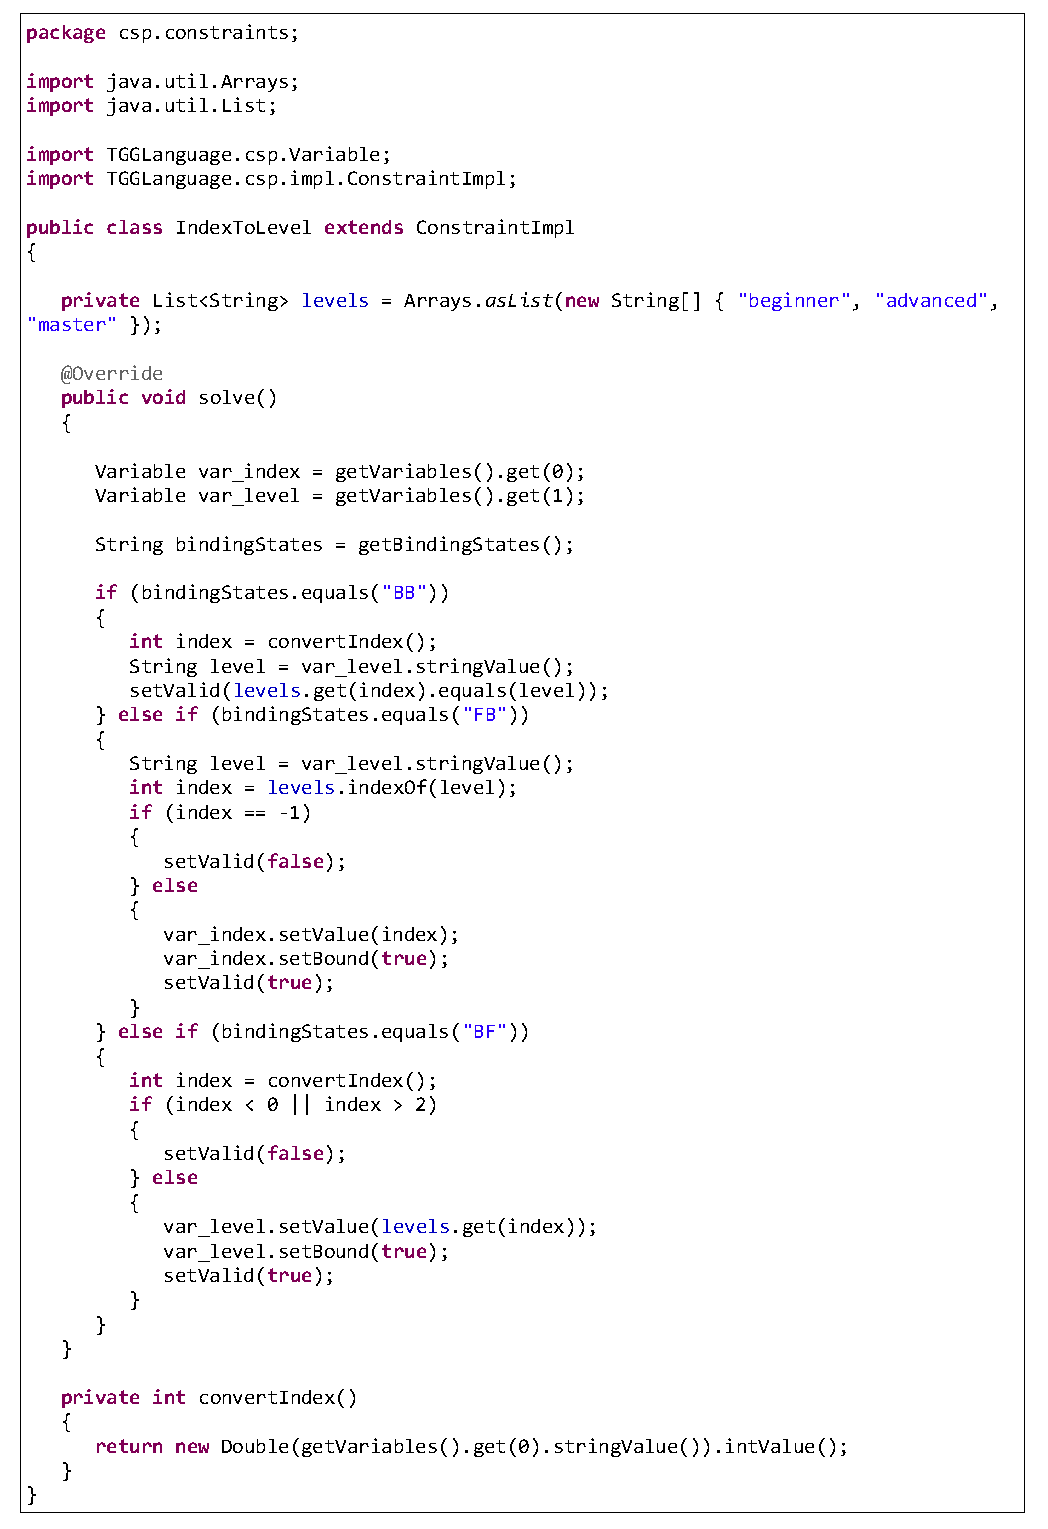
\includegraphics[height=0.64\textheight]{pics/tggBilder/transformation/tgg23}
\begin{lstlisting}[language=Java,backgroundcolor=\color{white}, keywordstyle={\bfseries\color{purple}}]
package csp.constraints;

import java.util.Arrays;
import java.util.List;

import TGGLanguage.csp.Variable;
import TGGLanguage.csp.impl.ConstraintImpl;

public class IndexToLevel extends ConstraintImpl {

  private List<String> levels = Arrays.asList(new String[] { "beginner",
      "advanced", "master" });


  public void solve(Variable<Integer> var_0, Variable<String> var_1){
    String bindingStates = getBindingStates(var_0, var_1);

    switch(bindingStates){
    case "BB":
      int indexBB = var_0.getValue().intValue();
      String level = var_1.getValue();
      setSatisfied(levels.get(indexBB).equals(level));
      break;
    case "BF":
     int indexFB = var_0.getValue().intValue();
      if (indexFB < 0 || indexFB > 2) {
        setSatisfied(false);
      } else {
        var_1.setValue(levels.get(indexFB));
        var_1.setBound(true);
        setSatisfied(true);
      }
      break;
    case "FB":
      String levelBF = var_1.getValue();
      int indexBF = levels.indexOf(levelBF);
      if (indexBF == -1) {
        setSatisfied(false);
      } else {
        var_0.setValue(indexBF);
        var_0.setBound(true);
        setSatisfied(true);
      }
      break;
    }

  }
}
\end{lstlisting}
  \caption{Implementation of our attribute constraint}
  \label{fig:indexToLevel}
\end{center}
\end{figure}

\clearpage

Now we shall create an instance model\footnote{Refer to Part II, Section 3 for review} of one of our languages, then transform it into an instance model of the
\emph{other} language as according to our TGG (i.e., perform a forward and backward transformation). Since dictionaries are a much simpler structure, lets start
with the ``backwards''\footnote{No direction implied} transformation, dictionary to learning box.

\begin{itemize}
\item[$\blacktriangleright$] Navigate to and open \texttt{Dictionary\-Language/model/Dictionary\-Language.ecore}. Create a dynamic instance of
\texttt{Dictionary} named \texttt{target.xmi}, and save it under \texttt{Learn\-ing\-Box\-To\-Dictionary\-In\-te\-gra\-tion/in\-stan\-ces/}
(Fig.~\ref{fig:create_instance_dict}).

\begin{figure}[htbp]
\begin{center}
  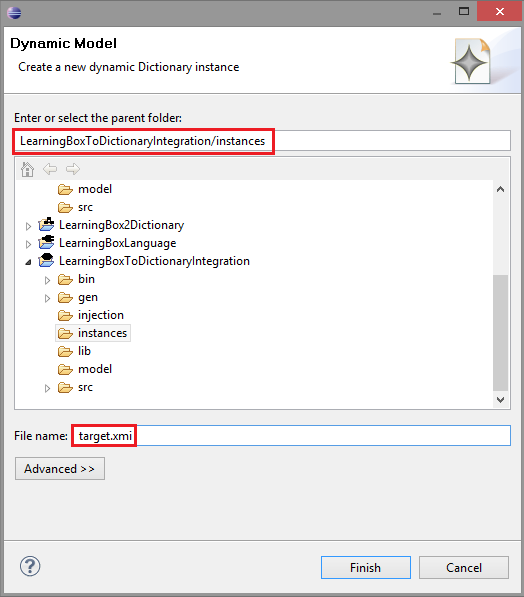
\includegraphics[width=0.7\textwidth]{tgg24}
  \caption{Create a dynamic instance of \texttt{Dictionary}}
  \label{fig:create_instance_dict}
\end{center}
\end{figure}

\item[$\blacktriangleright$] Open \texttt{target.xmi}, and edit the \texttt{Dictionary} properties by setting \texttt{Title} to \texttt{English Numbers}.

\item[$\blacktriangleright$] Create two child \texttt{Entry} objects. Set \texttt{Content} of the first to \texttt{one : eins} and its
\texttt{Level} as \texttt{beginner}. Set the second with \texttt{eleven : elf} and \texttt{advanced} (Fig.~\ref{fig:dictionaryxmi}).

\begin{figure}[htbp]
\begin{center}
  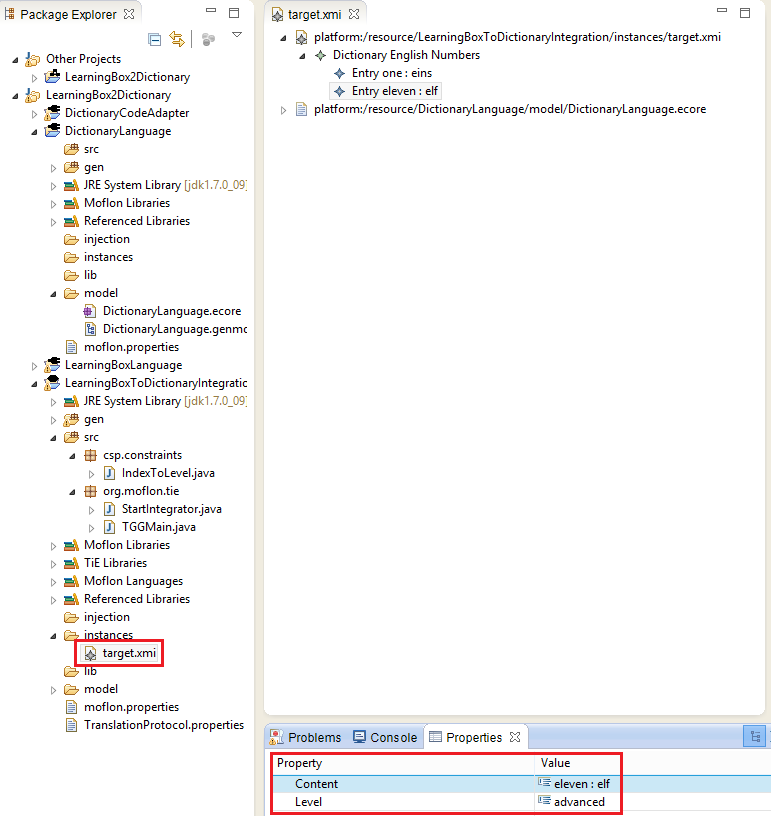
\includegraphics[width=\textwidth]{tgg26}
  \caption{Contents of the dictionary}
  \label{fig:dictionaryxmi}
\end{center}
\end{figure}

\item[$\blacktriangleright$] Run the main class, \texttt{TGGMain}, found in \texttt{LearningBox\-To\-Dictionary\-In\-te\-gra\-tion\-/src}, and refresh
\texttt{LearningBox\-To\-Dictionary\-In\-te\-gra\-tion/\-instances}.

\vspace{0.5cm}

\item[$\blacktriangleright$] Note the console error message, ``Unable to load instances/source.xmi, instances/source.xmi does not exist.'' This is referring to
the non-existent source file for the ``forward'' transformation - we'll fix this in a moment.
\end{itemize}

As you can see, our \texttt{Dictionary} has been translated backward to a \texttt{Box} with the same name (\texttt{English Numbers}) and containing three
\texttt{Par\-ti\-tions} (as specified in \texttt{Box\-To\-Dictionary\-Rule}). The two \texttt{Entry} objects have been translated to \texttt{Card} objects as
specified in \texttt{CartToEntryRule}. The \texttt{face} and the \texttt{back} of the \texttt{Card}s are consistent with the \texttt{content}
of the corresponding \texttt{Entry}, e.g. \texttt{card.face = ``Question : one''} and \texttt{card.back = ``Answer : eins''}. The indices of the partitions
containing the cards are also consistent with the level of the entry, i.e., \texttt{0} for \texttt{beginner}, and \texttt{1} for \texttt{advanced}.

\vspace{0.5cm}

Congratulations! You have successfully performed your first \emph{backward} transformation from your target model (dictionary) to your source (Learning box)
using TGGs! To show that the transformation is actually bidirectional however, lets edit the source model (thus resolving the error from above) and transform it
\emph{forward} to a new target model:

\begin{itemize}
\item[$\blacktriangleright$] Make a copy of \texttt{target.xmi\_BWD.xmi} (the result of the backward transformation)
and rename it to \texttt{source.xmi}.
  
\item[$\blacktriangleright$] Open \texttt{source.xmi} and create some new \texttt{Card} objects in the \texttt{Partition}s (e.g., create a new \texttt{Card}
with \texttt{Card.face = ``Question : two''}, \texttt{Card.back = ``Answer : zwei''} in \texttt{Partition 0}).

\item[$\blacktriangleright$] Run the \texttt{TGGMain.java} again and inspect the result of the forward transformation, target model
\texttt{source.xmi\_FWD.xmi}.

\end{itemize}


To end this chapter on TGGs, lets check out another feature of eMolfon, the integrator visualizer! This will let us view the visualization of the created
triple model.

\newpage

\begin{itemize}

\item[$\blacktriangleright$] Right-click on \texttt{corr\_BWD.xmi} and choose ``eMoflon $\rightarrow$ Start Integrator'' which will open the window depicted in
Fig.~\ref{fig:integrator_start}.

\vspace{0.5cm}

\begin{figure}[htbp]
\begin{center}
  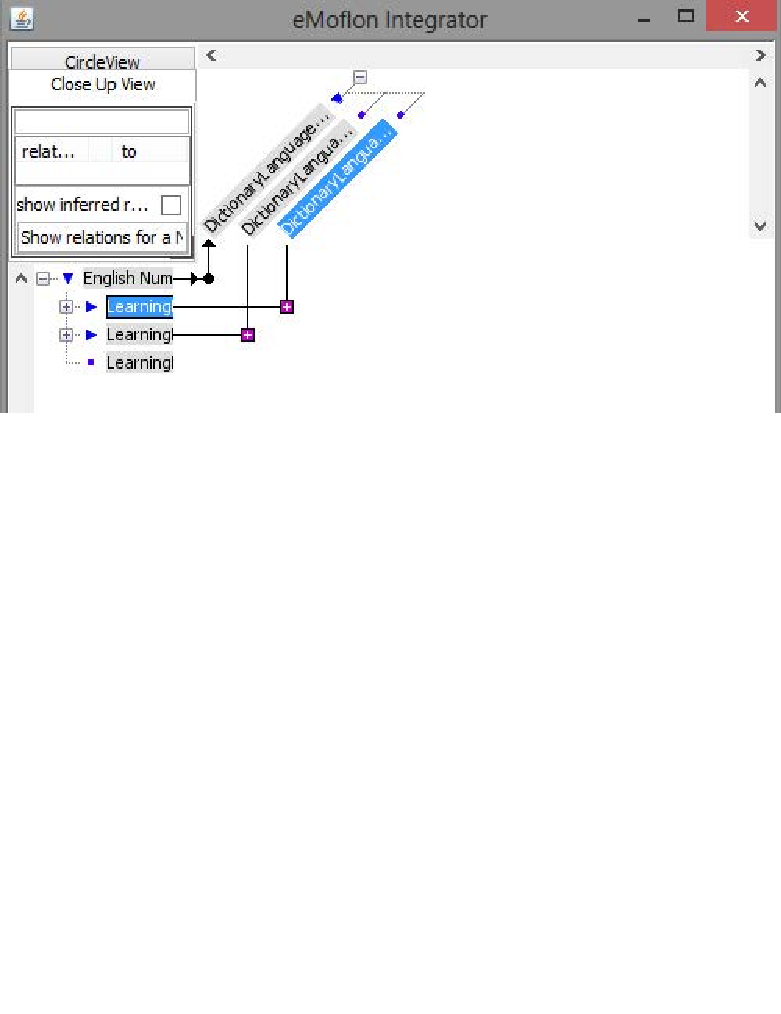
\includegraphics[width=0.7\textwidth]{integrator_start_view.pdf}
  \caption{Default view of the integrator}
  \label{fig:integrator_start}
\end{center}
\end{figure}

\item[$\blacktriangleright$] Drag and drop \texttt{protocol\_BWD.xmi} into the window. You will now see the controls explained in the lower part of the window 
(Fig.~\ref{fig:integrator_after_protocol}).

\begin{figure}[h!]
\begin{center}
  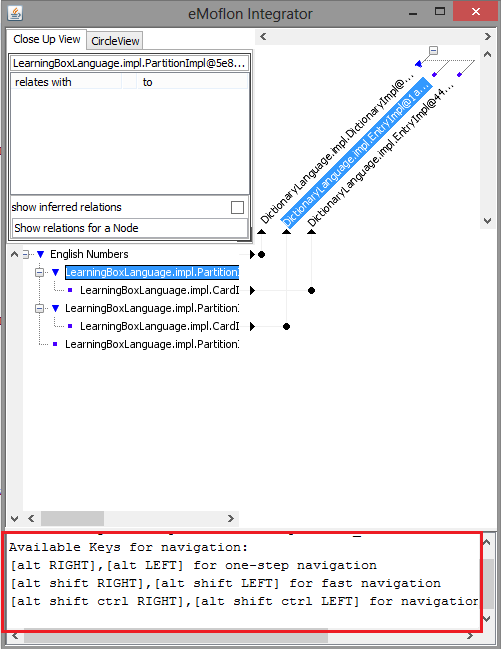
\includegraphics[width=0.6\textwidth]{integrator_after_protocol_insertion.png}
  \caption{Integrator after protocol insertion.}
  \label{fig:integrator_after_protocol}
\end{center}
\end{figure} 
\FloatBarrier

\item[$\blacktriangleright$] The integrator works as an ``offline'' debugger, working on the protocol (trace) of the transformation. You can use
\texttt{Alt+Right} to navigate forwards \emph{through} the transformation process, and \texttt{Alt+Left} to go backwards.  When you step through the
transformation, you will notice that some elements are highlighted with colours. These are the elements currently being processed. The colours have the
following definitions:
\begin{description}
  \item[Blue] The element is now about to be processed (is being ``looked at'').
  \vspace{0.5cm}
  \item[Yellow] The element cannot be transformed right now and has been queued for later transformation 
  (e.g., when transforming an Entry to a Card, the Box with partitions to put the 
  Card into must be translated first).
  \vspace{0.5cm}
  \item[Green] The object has just been created.
\end{description}

\end{itemize}


% Explain how works via INTEGRATOR (Part I) (NOTE. new interface?) 
\newpage
\section{Using the Integrator}
\genHeader
\label{sec:app_integrator}

% New interface? When reach this point, user will have a working TGG with 3 partitions, 3 entires. Explain the process via integrator

Let's check out another model visualization feature of eMolfon, the integrator! While you can ``see" the structure of a model with the graph viewer, the
integrator allows you to trace the transformation process. In other words, the integrator works as an ``offline'' debugger, working on the protocol (trace) of
the transformation.

\begin{itemize}

\item[$\blacktriangleright$] Right-click on \texttt{corr\_BWD.xmi} and choose ``eMoflon $\rightarrow$ Start Integrator'' which will open the window depicted in
Fig.~\ref{fig:integrator_start}.

\begin{figure}[htbp]
\begin{center}
  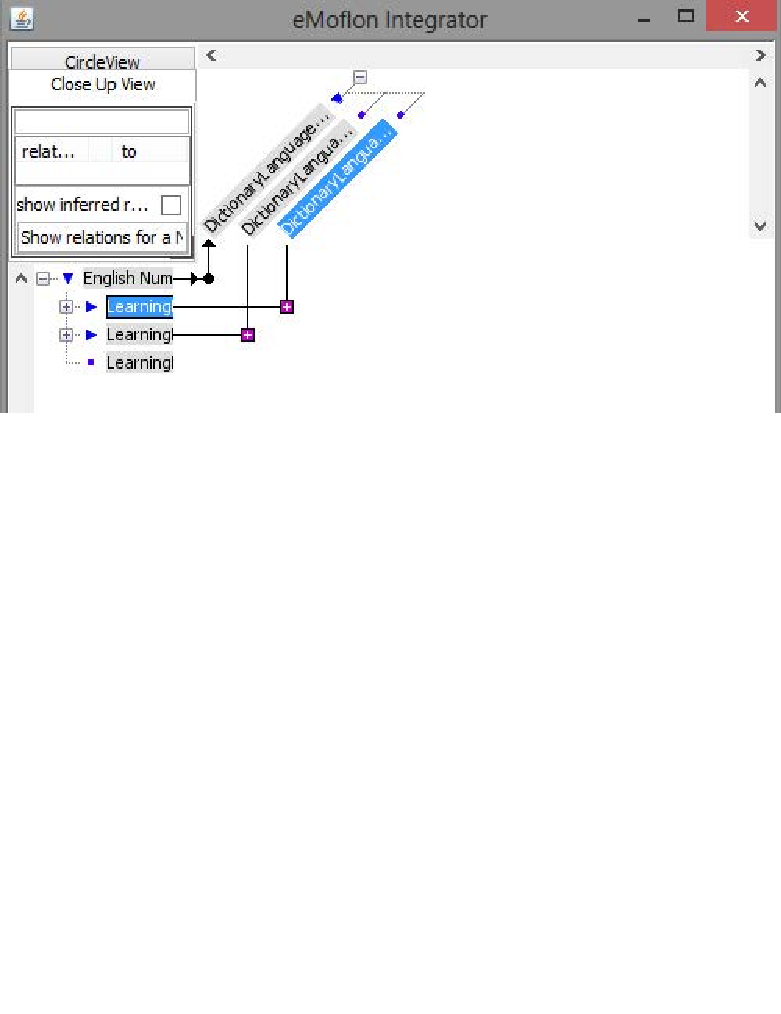
\includegraphics[width=0.7\textwidth]{integrator_start_view.pdf}
  \caption{Default view of the integrator}
  \label{fig:integrator_start}
\end{center}
\end{figure}

\item[$\blacktriangleright$] Drag and drop \texttt{protocol\_BWD.xmi} into the main window.\footnote{If the integrator window minimizes, press \texttt{alt+tab}
to re-activate it} You will now see the navigation controls explained in the lower part of the window (Fig.~\ref{fig:integrator_after_protocol}).

\begin{figure}[h!]
\begin{center}
  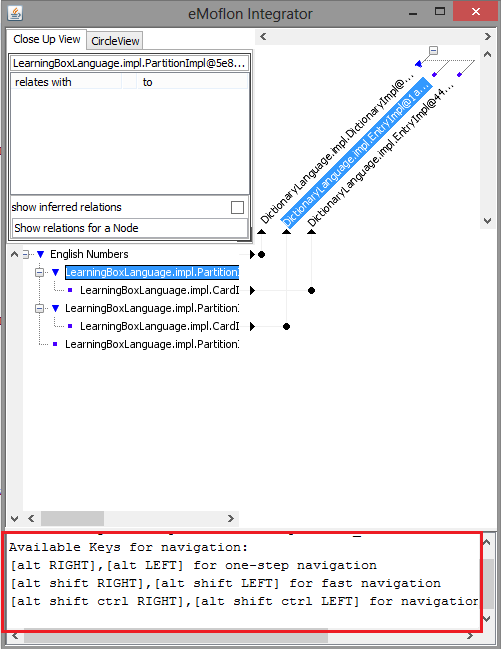
\includegraphics[width=0.6\textwidth]{integrator_after_protocol_insertion.png}
  \caption{Integrator after protocol insertion.}
  \label{fig:integrator_after_protocol}
\end{center}
\end{figure} 

\item[$\blacktriangleright$]  Starting at \texttt{Box}, you can use \texttt{Alt+Right} to navigate forwards \emph{through} the transformation process, and
\texttt{Alt+Left} to go backwards -- each step will appear with a small explanation in the small window below. {\bf end}

\item[$\blacktriangleright$] It lists which element it is currently working with, and then checks \emph{every} possible rule that could be applied. I.e.,
suppose we had two or three different \texttt{BoxToDictionary} rules, all defined slightly differently. What the TGG does, and the integrator displays, is how
each \texttt{card} is checked for each one of those rules. Even if the first rule is checked first and found applicable, it will \emph{still} check the other
two rules before moving on. If two rules are able to be applied, you will be prompted to choose.

\newpage

\item[$\blacktriangleright$] While you're stepping through the transformation, you will notice that some elements are highlighted with colours. These are the
elements currently being processed, and the colours have the following definitions:

\begin{description}
  \item[Blue] The element is now about to be processed (is being ``looked at'').
  
  \item[Yellow] The element cannot be transformed right now and has been queued for later transformation (i.e., when transforming an Entry to a Card, the Box
  with partitions to put the Card into must be translated first).
  
  \item[Green] The object has been created.
\end{description}

End Text.

\end{itemize}


% Introduce PROBLEM: well, even if it doesn't have capacity to deal with 4, 3 should still work. Introduce new rule
\newpage
\section{Extending your transformation}
\genHeader

At this point, we now have a working TGG triple to transform a \texttt{Dictionary} into a \texttt{Box} with three \texttt{partition}s, and a \texttt{Box} with
exactly three \texttt{Partition}s into \texttt{Dictionary}. The only potential problem is that a learning box with only three partitions may not be the most
useful studying tool. After all, the more partitions you have, the more practice you'll have with the cards by being quizzed again and again.

Let's try adding a fourth partition to \texttt{source.xmi} and run the TGG again. Given that we have a rule to transform three partitions, it should at least
complete a partial transformation on them, right? 

\begin{itemize}

\item[$\blacktriangleright$] Add a \texttt{partition3} with one \texttt{card} to your \texttt{source.xmi} so that it resembles
Fig.~\ref{eclipse:fourthPartitionStart}. Don't forget to set the partition's \texttt{previous} attribute to \texttt{partition0}, and \texttt{partition2.next} to
\texttt{partition3}.

\begin{figure}[htbp]
\begin{center}
  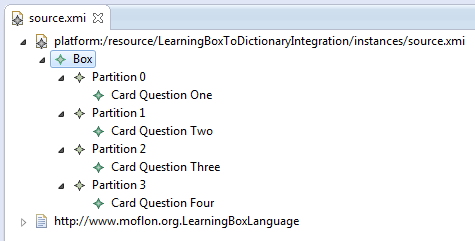
\includegraphics[width=0.7\textwidth]{eclipse_fillFourthPartition}
  \caption{Adding a fourth partition to \texttt{Box}}
  \label{eclipse:fourthPartitionStart}
\end{center}
\end{figure}

\item[$\blacktriangleright$] An error should appear in the eMolfon console window stating that there was a problem translating your new partition, but the
forward transformation was still able to finish. In fact, if you open \texttt{source.xmi\_FWD.xmi}, you'll be able to confirm the \texttt{English Numbers
Dictionary} was still created and includes your newest card! Let's run the integrator on \texttt{corr\_fwd.xmi} once more to find out exactly how this worked.

\item[$\blacktriangleright$] Start once again with \texttt{Box}, and proceed until the integrator reaches your fourth partition. You'll notice that it
first delays processing the \texttt{partition} as it cannot find a valid rule candidate.\footnote{The message 'Possible Rule Candidate(s): ' will not be
displayed here as the element is simply ignored} Instead, it goes ahead and tries to process \texttt{card}.

\item[$\blacktriangleright$] Here the transformation is able to find a valid rule but opts to delay the action as \texttt{CardToEntryRule} needs the black
\texttt{partition} element from the \texttt{partition} to complete.\footnote{Review the \texttt{source} of your rule if confused}

\item[$\blacktriangleright$] Returning to \texttt{partition}, the transformation detects an endlessly repeating result of not finding a valid rule and so,
terminates the action (Fig.~\ref{eclipse:integrator_debugSuccess}). Instead of canceling the entire transformation however, it takes an optimistic approach and
tries to solve \texttt{Question Four} \emph{anyway}. The action succeeds!

\begin{figure}[htb]
\begin{center}
  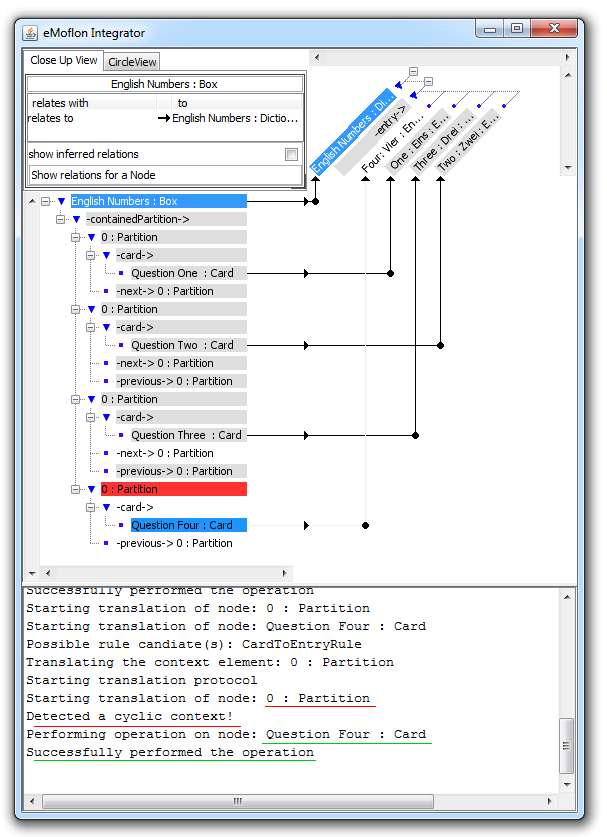
\includegraphics[width=0.7\textwidth]{eclipse_integratorDebug}
  \caption{Detecting errors with the integrator}
  \label{eclipse:integrator_debugSuccess}
\end{center}
\end{figure}

\item[$\blacktriangleright$] The final task is to try and resolve each of the link variables, but it fails to find rule candidates for any of \texttt{previous},
\texttt{containedPartition}, or \texttt{next}, and so the transformation ends.

\clearpage

We're now presented with a dilemma. This rule, while giving us an error, \emph{works}! Our goal was never the to be able to put an \texttt{Entry} into
partitions with indexes greater than two,\footnote{As resolved in the \texttt{IndexTolevel} implementation} but simply to be able to put any \texttt{card} into
a \texttt{Dictionary}. So why not leave our transformation like this?

\vspace{0.5cm}

In short, it just feels \emph{dirty}. It just cooperates with you and manages to get the job done, and that's it. Instead, let's add a new rule to handle this
additional structure. We could keep things simple by extending the existing \texttt{BoxToDictionaryRule} by connecting a fourth partition, what if we wanted a
fifth one? A sixth? As you can see, this obviously won't work -- there will always be the potential for a \texttt{n+1}th card in an \texttt{n}-sized
box. 

\vspace{0.5cm}

While building this rule, keep in mind that the goal is to simply handle any additional elements and their connecting link variables in \texttt{Box}. This means
we don't need to create any new \emph{correspondence types} to \texttt{Dictionary}.

\end{itemize}

\jumpDual{allCards vis}{allCards tex}


\newpage
\hypertarget{allCards vis}{}
\subsection{AllOtherPartitionsRule}
\genHeader

\begin{itemize}

\item[$\blacktriangleright$] Create a new rule \texttt{AllOtherPartitionsRule}, and complete it according to \Cref{fig:ea_AllOtherPartitionsRuleComplete}.


\begin{figure}[htbp]
\begin{center}
  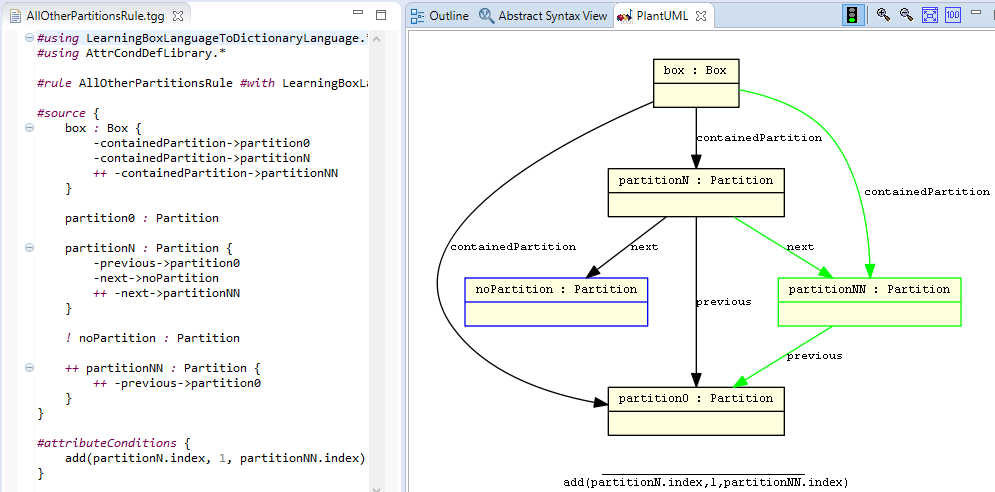
\includegraphics[width=\textwidth]{ea_AllOtherPartitionsRule}
  \caption{The completed \texttt{AllOtherPartitionsRule}}
  \label{fig:ea_AllOtherPartitionsRuleComplete}
\end{center}
\end{figure}

\item[$\blacktriangleright$] As you can see, this rule doesn't assume to know the final \texttt{partition} in the transformation. 
It matches the \texttt{n}th partition as the partition without any next partition, then connects a new \texttt{n+1}th partition to \texttt{n} and \texttt{partition0} (clear as every partitions previous is \texttt{partition0}).
Note that TGG transformations assume that the models are valid, i.e., have the expected structure (in our case meaning that the learning box is correctly ``wired'').\footnote{This should actually be formalised with a set of metamodel constraints that must be checked before a transformation is run, but we've omitted this here to simplify things.}  
Remember that ``blue'' means ``negative''.

\item[$\blacktriangleright$] Generate code for your improved TGG and re-run the transformation. 
It should work now without any error message.
Inspect the protocol to understand what happened.

\item[$\blacktriangleright$] Go ahead and add as many \texttt{partition}s and \texttt{card}s as you like to your model instance.
Your TGG is now also able to handle a \texttt{box} with any number of \texttt{partition}s beautifully.
For five partitions all with cards, the protocol gets quite interesting and is no longer a flat tree.
Try it out! 

\end{itemize}



%%% Local Variables: 
%%% mode: latex
%%% TeX-master: "../src/TGG_mainFile"
%%% End: 


\newpage
\hypertarget{allCards tex}{}
\subsection{AllOtherCardsRule}
\texHeader

\begin{itemize}

\item[$\blacktriangleright$] Right click on the \texttt{rules} folder again and create \texttt{AllOtherCardsRule}. Complete the rule until your file resembles
Fig.~\ref{fig:eclipse_allOtherCardsRule}.

\vspace{0.5cm}

\begin{figure}[htbp]
\begin{center}
  \includegraphics[width=0.7\textwidth]{eclipse_allOtherCardsRule}
  \caption{A complete \texttt{AllOtherCardsRule}}
  \label{fig:eclipse_allOtherCardsRule}
\end{center}
\end{figure}

\item[$\blacktriangleright$] You'll notice that \texttt{box} and \texttt{partition0} have been established as `black' objects -- this rule may only be evaluated
when these objects are already known (and simply need to be adjusted), so we can use their values from the context of the transformation.

\vspace{0.5cm}

\item[$\blacktriangleright$] A second partition, \texttt{partitionN}, has also been established from the context. It represents the \texttt{n}th or last
partition in a \texttt{box} (with an index of 2 or higher), whose \texttt{next} reference will be updated in order to provide an access
link to the newest element, \texttt{partitionNN}.

\newpage

\item[$\blacktriangleright$] Given that the \texttt{add(a,b,c)} syntax is \texttt{a+b=c}, the sole constraint of this rule sets the \texttt{index} of the
\texttt{n+1}th partition so that the \texttt{partition}s are still listed in order.

\vspace{0.5cm}

\item[$\blacktriangleright$] That's it! Save and build your package explorer, then run the TGG again with the `extra' \texttt{partition} to confirm it worked!
You are now free to add as many \texttt{partition}s and \texttt{card}s to \texttt{source.xmi} -- the transformation is now able to elegantly handle them all.

\vspace{0.5cm}

\item[$\blacktriangleright$] Be sure to check out how this rule is implemented in eMoflon's visual specification with Fig.~\ref{fig:ea_allOtherCardsRule} from
the previous section.

\end{itemize}


% Not needed? remind users to check out and read the protocol in their syyntaxes for detail or run the integrator.
% \newpage
\section{The Protocol Explained}
\genHeader

% files are saved and built/refereshed in the Eclipse workspace.

Now that everything is working correctly, let's return to one of the generated protocol files and quickly review what happens in greater detail. Though it looks
scary, this file can prove to be useful if the integrator was ever to fail again, or if you simply wanted to know more detail about what happened during the
transformation process.

\ldots



%  --------------- UNDER CONSTRUCTION (DELAYED RELEASE) --------------------------------------------------------------------------------
%\newpage
\section{Integrator Breakpoints**}
\genHeader

{\bf Under Construction}

\vspace{0.5cm}

TASKS:

\begin{itemize}
  \item Streamline the breakpoint process (so user does not have to implement code re: original instructions)
  
  \item Example: Find out when FORALLCARDSRULE is executed in place of CARDTOENTRYRULE
  
  \item Explain: if there were ever two different applicable rules, you could set up a breakpoint and then be prompted to choose which one you'd like to use.
  Useful for testing?

\end{itemize}


% --------------- UNDER CONSTRUCTION (DELAYED RELEASE) --------------------------------------------------------------------------------
% Synchronization (To deal with data loss: i.e., from partition to entry and back : no way to put say, fourth partition BACK in fourth)
%\newpage
\section{Model Synchronization**}
\genHeader

{\bf Under Construction}

At this point you have successfully created a trio of rules that can transform a \texttt{box} (with an undetermined number of \texttt{partition}s which can
contain an unkown number of \texttt{card}s) \emph{forwards} into a single \texttt{dictionary} able to store an unlimited number of \texttt{entry} elements.
Unfortunately, there would be unavoidable data loss if you attempted transform data \emph{backwards} from \texttt{dictionary}.

Suppose you first ran the TGG on a \texttt{source.xmi} graph with five \texttt{partition}s, each containing three \texttt{Card}s. According to our
\texttt{IndexToLevel} implementation, the \texttt{card}s would be transformed as (1) three ``beginner'' entries, (2) three ``advanced'' entries, and (3)
nine ``master'' entries. If you were to now run the TGG on the generated \texttt{target} graph and inspect the output, you would have a \texttt{box} with
only three partitions of size nine, three, and three, respectively. There is no possible way to achieve the original construction of the other two partitions!

\vspace{1cm}

TASKS:

\begin{itemize}
  \item example to find out/explain/resolve model synchronization
\end{itemize}



% Conclusion to forward users onto other parts
\section{Conclusion and next steps}
\genHeader

\vspace{0.5cm}

Absolutely amazing work -- you've mastered Part IV of the eMoflon handbook! You've learnt the key points of Triple Graph Grammars (TGGs) and \emph{bidirectional} transformations, and now know how to set up a TGG consisting of a schema and a set of rules. 
With these basic skills, you should be able to tackle quite a few bidirectional transformations using TGGs.

For detailed descriptions on the upcoming and previous parts of this handbook, please refer to Part 0, which can be found at 

\dlPartZero.

Cheers!


%%% Local Variables: 
%%% mode: latex
%%% TeX-master: "TGG_mainFile"
%%% End: 


\newpage
\chapter{Triple Graph Grammars glossary}

\begin{description}

\item[Correspondence Types] Connect classes of the source and target metamodels.

\item[Graph Triples] Consist of connected source, correspondence, and target components.

\item[Link or correspondence Metamodel] Comprised of all correspondence types.

\item[Monotonic] In this context, non-deleting.

\item[Operationalization] The process of deriving step-by-step executable instructions from a declarative specification that just states what the outcome should
be but not how to achieve it.

\item[Triple Graph Grammars (TGG)] Declarative, rule-based technique of specifying the simultaneous evolution of three connected graphs.

\item[TGG Schema] The metamodel triple consisting of the source, correspondence (link), and target metamodels.

\end{description}

% -- References
\newpage \genHeader
\phantomsection
\addcontentsline{toc}{section}{References}
\renewcommand*{\bibname}{References}
\bibliographystyle{plain}  
\bibliography{../../06_miscellaneous/commonFiles/references}

% Glossary?
% \newpage
\chapter{Triple Graph Grammars glossary}

\begin{description}

\item[Correspondence Types] Connect classes of the source and target metamodels.

\item[Graph Triples] Consist of connected source, correspondence, and target components.

\item[Link or correspondence Metamodel] Comprised of all correspondence types.

\item[Monotonic] In this context, non-deleting.

\item[Operationalization] The process of deriving step-by-step executable instructions from a declarative specification that just states what the outcome should
be but not how to achieve it.

\item[Triple Graph Grammars (TGG)] Declarative, rule-based technique of specifying the simultaneous evolution of three connected graphs.

\item[TGG Schema] The metamodel triple consisting of the source, correspondence (link), and target metamodels.

\end{description}

\end{document}